\documentclass[a4paper,12pt]{article}
\usepackage[utf8]{inputenc}
\usepackage[T2A]{fontenc}
\usepackage[russian]{babel}
\usepackage{amsmath, amssymb, amsfonts}
\usepackage{graphicx}
\usepackage{geometry}
\usepackage{hyperref}
\usepackage{cite}
\usepackage{float}
\usepackage{subcaption} % если нужны подрисуночные подписи

\geometry{left=1cm, right=1cm, top=1cm, bottom=1cm}

\title{\textbf{Электродинамический анализ волнового двигателя MenDrive:
механизм слабой компенсации тяги противосилой на витке возбуждения
и проблема сохранения импульса в неоднородных средах}}
\author{А.Ю. Дроздов}
\date{\today}

\begin{document}

\maketitle

\begin{abstract}
В работе представлено строгое численное решение краевой задачи для уравнений
Максвелла в трёхслойной асимметричной структуре (металл/вакуум/феррит) с учётом
конечной проводимости и магнитных потерь. На основе полной динамической формулы
пондеромоторной силы (И.Е. Тамм, \S 18, ф-ла 18.9) вычислены все компоненты силы,
действующей на стенки резонатора. Показано, что в асимметричной среде силы на
металлическую и ферритовую стенки не компенсируют друг друга, что приводит к
возникновению результирующей тяги порядка $10^2$--$10^3$ Н/кВт. Проведён детальный
анализ силы реакции на виток возбуждения: обнаружено, что степень компенсации
тяги противосилой витка составляет $\eta \approx 10^{-5}$--$10^{-2}$ в зависимости
от дисперсионной ветви. Выявлен физический механизм слабой компенсации: в режимах
с высокой удельной тягой эффективное волновое сопротивление моды $Z_{\text{eff}} \ll 1$,
что приводит к пренебрежимо малой силе Ампера на виток. Обсуждается связь с
парадоксом 4/3 и работами Ф. Рорлиха о ковариантном определении импульса.
Предлагается обобщённый закон сохранения импульса для неоднородных сред с учётом
внутренних поверхностных интегралов тензора натяжений на границах раздела.

\textbf{Ключевые слова:} пондеромоторные силы, асимметричный резонатор, закон
сохранения импульса, волновое сопротивление, дисперсионные ветви, тензор
натяжений Максвелла, парадокс 4/3.
\end{abstract}

\section{Введение}

Проблема создания двигательных систем без выброса рабочего тела стимулирует
поиск новых электродинамических эффектов. Концепция волнового двигателя с
внутренним расходом энергии (MenDrive), предложенная Ф.Ф. Менде \cite{Mende},
базируется на генерации тяги за счёт асимметрии пондеромоторных сил в
композитной структуре с различными электромагнитными свойствами стенок.

Критический анализ \cite{Karavashkin, Drozdov} указывал на необходимость
строгого учёта закона сохранения импульса (И.Е. Тамм, \S 105 \cite{Tamm}).
В частности, оставался открытым вопрос о компенсации тяги силой реакции
на источнике питания.

Эксперименты с EmDrive (NASA/Таймар, 2015--2016) показали, что в симметричных
резонаторах тяга полностью компенсируется противосилой на витках возбуждения
\cite{Tajmar2016}. Однако конфигурация MenDrive принципиально отличается:
асимметрия материалов (металл/феррит) создаёт условия для слабой компенсации.

Цель данной работы:
\begin{enumerate}
    \item Построить самосогласованную электродинамическую модель MenDrive
    на основе строгого решения уравнений Максвелла;
    \item Вычислить полный набор компонент пондеромоторной силы с использованием
    динамической формулы Тамма (\S 18, ф-ла 18.9);
    \item Детально проанализировать силу реакции на витке возбуждения и выявить
    механизм её слабости по сравнению с тягой;
    \item Обсудить связь с парадоксом 4/3 и работами Ф. Рорлиха о ковариантном
    определении импульса электромагнитного поля;
    \item Предложить обобщённый закон сохранения импульса для неоднородных сред
    с учётом внутренних поверхностных интегралов тензора натяжений.
\end{enumerate}

\section{Математическая модель}

\subsection{Геометрия системы}

Рассматривается трёхслойная структура в декартовых координатах $(x, y, z)$:

\begin{itemize}
    \item \textbf{Область 1} ($x \leq -A$): металл с параметрами 
    $\varepsilon_m \approx 1$, $\mu_m = 1$, 
    $\sigma_m = 5.8 \times 10^{17}$ с$^{-1}$ (СГС);
    \item \textbf{Область 2} ($-A \leq x \leq +A$): вакуум 
    ($\varepsilon_0 = \mu_0 = 1$);
    \item \textbf{Область 3} ($x \geq +A$): металл (правый проводник) с параметрами
    $\varepsilon_m \approx 1$, $\mu_m = 1$, $\sigma_m = 5.8 \times 10^{17}$ с$^{-1}$ (СГС).
\end{itemize}

Параметры: $A = 0.5$ см, толщина проводников $h = 0.1$ см.

\subsection{Уравнения Максвелла в симметричной форме}

Используется симметричная форма уравнений Максвелла с магнитными токами:

\begin{equation}
\begin{cases}
\text{rot} \vec{E} = -\frac{1}{c}\frac{\partial \vec{B}}{\partial t} 
- \frac{4\pi}{c}\vec{j}_m \\
\text{rot} \vec{H} = \frac{1}{c}\frac{\partial \vec{D}}{\partial t} 
+ \frac{4\pi}{c}\vec{j}_e
\end{cases}
\label{eq:maxwell_symmetric}
\end{equation}

где $\vec{j}_m$ --- плотность магнитного тока, вводимая для описания
намагниченности феррита.

Поле ищется в виде $\vec{F}(x) e^{i(k_z z - \omega t)}$ с комплексным
волновым числом $k_z = k_z' + i k_z''$. При условии $\partial/\partial y = 0$ 
($k_y = 0$) уравнения разделяются на TE- и TM-моды.

\subsection{Граничные условия и характеристическое уравнение}

На границах $x = \pm A$ выполняются стандартные условия непрерывности
тангенциальных компонент $\vec{E}$ и $\vec{H}$:

\begin{equation}
E_{t}^{(1)} = E_{t}^{(2)}, \quad H_{t}^{(1)} = H_{t}^{(2)}, \quad
D_{n}^{(1)} = D_{n}^{(2)}, \quad B_{n}^{(1)} = B_{n}^{(2)}
\label{eq:boundary_conditions}
\end{equation}

Подстановка общих решений волновых уравнений в граничные условия приводит
к системе линейных уравнений для амплитудных коэффициентов:

\begin{equation}
\mathbf{M}(k_z, \omega) \cdot \vec{C} = 0
\label{eq:linear_system}
\end{equation}

Условие существования нетривиального решения:

\begin{equation}
\det \mathbf{M}(k_z, \omega) = 0
\label{eq:characteristic}
\end{equation}

Определитель символьно вычислен в SageMath и скомпилирован в C-библиотеку
(точность \texttt{float128}). Поиск корней осуществляется методом Ньютона. 
Для каждого $\omega$ обнаруживается 4--12 дисперсионных ветвей.

\section{Методика расчёта пондеромоторных сил}

\subsection{Полная динамическая формула Тамма}

\textbf{Критически важно:} для расчёта сил в динамических полях необходимо
использовать формулу 18.9 из \S 18 книги Тамма \cite{Tamm}, а не формулу 17.5, 
которая верна только для статики.

В симметричной форме с магнитными токами плотность пондеромоторной силы:

\begin{equation}
\vec{f} = \rho_e \vec{E} + \frac{1}{c}[\vec{j}_e \times \vec{B}] 
+ \rho_m \vec{H} + \frac{1}{c}[\vec{j}_m \times \vec{D}] 
+ \vec{f}_{\text{Abraham}} + \vec{f}_{\text{conv}}
\label{eq:tamm18.9}
\end{equation}

\textbf{Важно:} формула (18.9) справедлива для динамических полей, в отличие 
от статической формулы (17.5). В симметричной форме с магнитными токами 
учитываются все компоненты силы.

\subsection{Компоненты силы}

В коде реализован расчёт следующих усреднённых по периоду компонент:

\begin{enumerate}
    \item \textbf{Сила Лоренца на токи проводимости:}
    $F_{jeB} \sim \text{Re}[\vec{j}_e \times \vec{B}^*]$

    \item \textbf{Сила на магнитные токи:} 
    $F_{jmD} \sim \text{Re}[\vec{j}_m \times \vec{D}^*]$ (критично для феррита)

    \item \textbf{Силы Абрагама:} действующие на векторы намагниченности
    $\vec{I}$ и поляризации $\vec{P}$ через роторы полей:
    \begin{equation}
    \vec{F}_I \sim \vec{I} \times \text{rot}\vec{B}, \quad
    \vec{F}_P \sim \vec{P} \times \text{rot}\vec{E}
    \end{equation}

    \item \textbf{Конвективные члены:} связанные с градиентами полей на границах:
    \begin{equation}
    \vec{f}_{\text{conv}} \sim (\vec{I}\nabla)\vec{H}, \quad (\vec{P}\nabla)\vec{E}
    \end{equation}

    \item \textbf{Натяжения Максвелла:} давление нормальных и тангенциальных
    компонент:
    \begin{equation}
    p_{D_n} = \frac{D_n^2}{8\pi\varepsilon}, \quad
    p_{H_t} = \frac{H_t^2}{8\pi}
    \end{equation}
\end{enumerate}

Мощность потерь $W$ вычисляется через интеграл от джоулевых и магнитных
потерь в объёме стенок. Удельная тяга: $\mathcal{T} = F_x / W$ [Н/кВт].


\section{Методика параметрического сканирования и идентификация дисперсионных ветвей}

\subsection{Поиск корней характеристического уравнения}

Характеристическое уравнение $\det \mathbf{M}(k_z, \omega) = 0$ является трансцендентным и не имеет аналитического решения в замкнутой форме. Для поиска комплексных корней $k_z = k_z' + i k_z''$ при фиксированной частоте $\omega$ применяется двухстадийный численный алгоритм:

\begin{enumerate}
    \item \textbf{Графическая локализация:} Строится сетка значений в комплексной плоскости $(k_z', k_z'')$ и вычисляются изолинии $\text{Re}[\det \mathbf{M}] = 0$ и $\text{Im}[\det \mathbf{M}] = 0$. Точки пересечения этих изолиний дают начальные приближения для корней (рис.~\ref{fig:det_contours}).

    \item \textbf{Итерационное уточнение:} Каждое начальное приближение уточняется методом Ньютона для комплексной функции:
    \begin{equation}
    k_z^{(n+1)} = k_z^{(n)} - \frac{\det \mathbf{M}(k_z^{(n)})}{\partial \det \mathbf{M} / \partial k_z \big|_{k_z^{(n)}}}
    \label{eq:newton_complex}
    \end{equation}
    Критерий сходимости: $|\det \mathbf{M}| < 10^{-20}$.
\end{enumerate}

\begin{figure}[h]
\centering
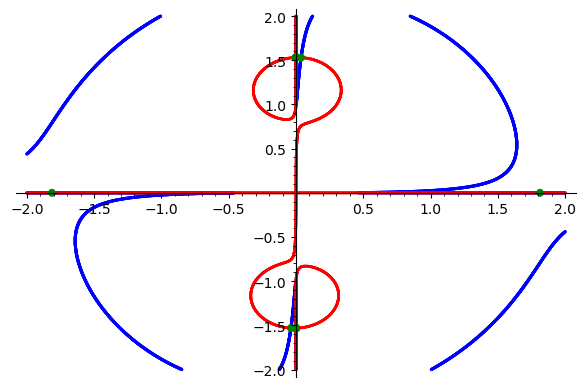
\includegraphics[width=0.9\textwidth]{det_re_im_isolines.png}
\caption{Изолинии действительной (синие) и мнимой (красные) компонент определителя в комплексной плоскости $k_z$ для $\omega = 10^5$ рад/с. Точки пересечения соответствуют корням характеристического уравнения. Зелёные маркеры --- уточнённые корни методом Ньютона.}
\label{fig:det_contours}
\end{figure}

\subsection{Сканирование по частоте и сопоставление ветвей}

Для построения дисперсионных зависимостей проводится сканирование по частоте $\omega$ в диапазоне $10^5$--$10^6$ рад/с с логарифмическим шагом. На каждом шаге находится набор корней $\{k_z^{(j)}(\omega)\}$.

\textbf{Проблема:} при изменении $\omega$ корни могут «перескакивать» между ветвями, и необходимо автоматически сопоставлять корни на соседних частотах.

\textbf{Решение:} вводится метрика близости корней, учитывающая:
\begin{itemize}
    \item Расстояние в комплексной плоскости: $d_k = |k_z^{(i)} - k_z^{(j)}|$
    \item Близость параметров затухания в средах:
    \begin{equation}
    d_K = w_K \left( |K_{\text{left}}^{(i)} - K_{\text{left}}^{(j)}| +
    |K_{\text{vac}}^{(i)} - K_{\text{vac}}^{(j)}| +
    |K_{\text{right}}^{(i)} - K_{\text{right}}^{(j)}| \right)
    \end{equation}
    где $K = \sqrt{k_0^2 \varepsilon \mu - k_z^2}$ --- поперечное волновое число в соответствующей среде.
\end{itemize}

Общая метрика: $d = \sqrt{d_k^2 + d_K^2}$. Если $d < d_{\text{threshold}}$, корни считаются принадлежащими одной ветви.

\subsection{Идентификация дисперсионных ветвей}

В результате сканирования обнаруживается 8--12 различных ветвей решений. Каждая ветвь характеризуется уникальным набором параметров:

\begin{table}[h]
\centering
\caption{Классификация основных дисперсионных ветвей}
\label{tab:branches}
\begin{tabular}{@{}cccccc@{}}
% \toprule
\textbf{Ветвь} & \textbf{$\text{Re}(k_z)$, см$^{-1}$} & \textbf{$\text{Im}(k_z)$, см$^{-1}$} & \textbf{$L_z$, см} & \textbf{Тип моды} & \textbf{Уд. тяга, Н/кВт} \\
% \midrule
Branch 0 & $-1.03$ & $-38.6$ & $0.013$ & Поверхностная & $-963$ \\
Branch 4 & $-1.2 \dots -2.2$ & $-129.6$ & $0.004$ & Осцилляторная & $-313$ \\
Branch 5 & $-0.038 \dots -0.012$ & $-1.53 \dots -1.56$ & $0.33$ & Распространяющаяся & $-2006$ \\
% \bottomrule
\end{tabular}
\end{table}

\textbf{Ключевые различия:}

\begin{itemize}
    \item \textbf{Branch 5:} Малое затухание вдоль $z$ ($|\text{Im}(k_z)| \approx 1.5$ см$^{-1}$), длина затухания $L_z = 1/(2|\text{Im}(k_z)|) \approx 0.33$ см. Поле распространяется на несколько сантиметров вдоль резонатора. Это режим, близкий к распространяющейся волне с умеренными потерями.

    \item \textbf{Branch 4:} Сильное затухание ($|\text{Im}(k_z)| \approx 130$ см$^{-1}$), $L_z \approx 0.004$ см = 40 мкм. Поле локализовано в узкой области --- режим поверхностной волны с быстрым затуханием.

    \item \textbf{Branch 0:} Промежуточный случай с $|\text{Im}(k_z)| \approx 39$ см$^{-1}$.
\end{itemize}

\subsection{Детальный анализ ветви 5}

Ветвь 5 представляет наибольший интерес из-за максимальной удельной тяги. На рис.~\ref{fig:branch5_analysis} показаны результаты параметрического анализа.

\begin{figure}[h]
\centering
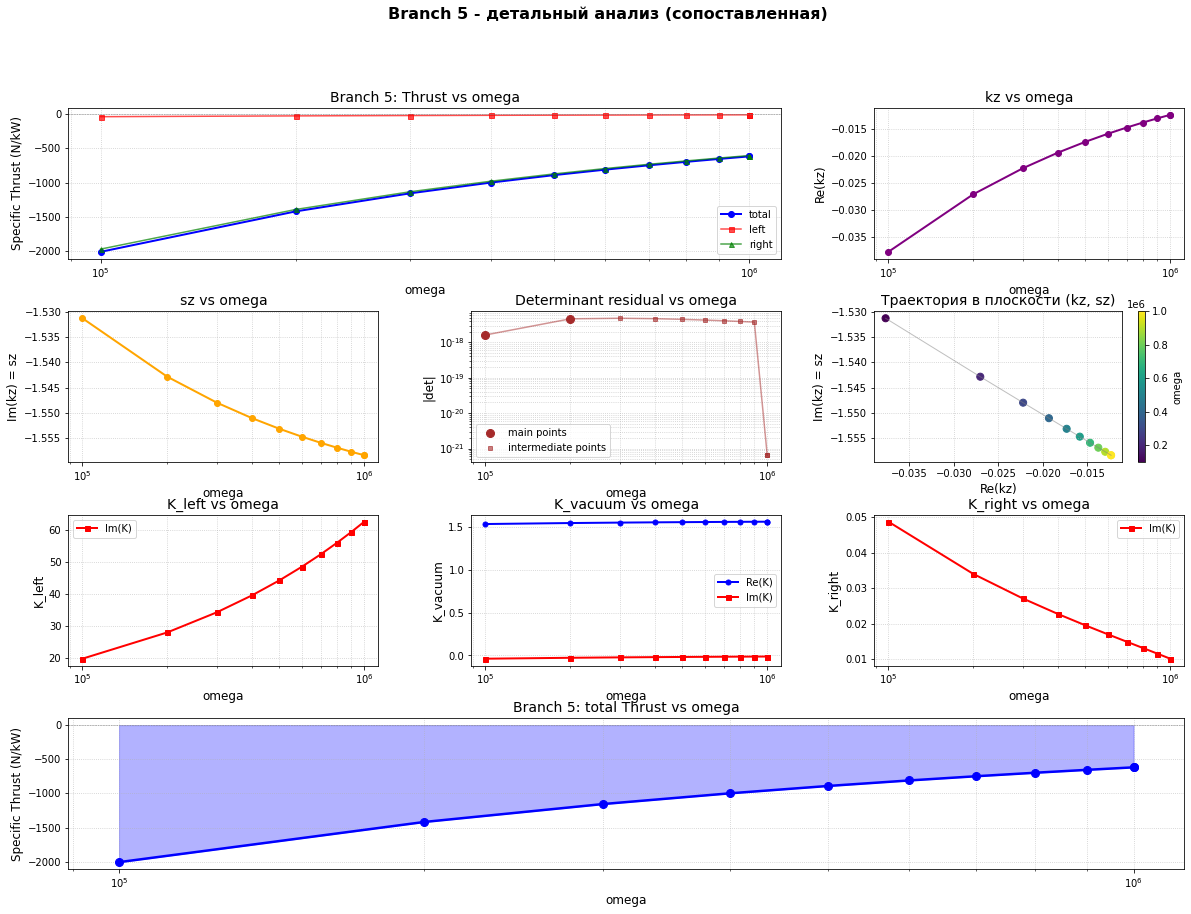
\includegraphics[width=\textwidth]{branch5_details.png}
\caption{Детальный анализ ветви 5: (а) зависимость удельной тяги от частоты; (б) траектория корня в комплексной плоскости $k_z$; (в) невязка детерминанта; (г) параметры затухания $K$ в трёх средах.}
\label{fig:branch5_analysis}
\end{figure}

\textbf{Основные наблюдения:}

\begin{enumerate}
    \item \textbf{Тяга:} Удельная тяга монотонно уменьшается по абсолютной величине с ростом частоты: от $-2006$ Н/кВт при $\omega = 10^5$ рад/с до $-618$ Н/кВт при $\omega = 10^6$ рад/с.

    \item \textbf{Дисперсия:} $\text{Re}(k_z)$ изменяется незначительно ($-0.038 \dots -0.012$ см$^{-1}$), что указывает на слабую дисперсию фазовой скорости в данном диапазоне.

    \item \textbf{Затухание:} $\text{Im}(k_z)$ также слабо зависит от частоты, что подтверждает устойчивость режима.

    \item \textbf{Точность:} Невязка $|\det \mathbf{M}|$ не превышает $10^{-18}$ во всём диапазоне, что подтверждает корректность численного решения.

    \item \textbf{Параметры $K$:} Модули $|K_{\text{left}}|$, $|K_{\text{vac}}|$, $|K_{\text{right}}|$ демонстрируют различное поведение, отражая асимметрию затухания полей в металле, вакууме и феррите.
\end{enumerate}

\subsection{Детальный анализ ветви 4}

Ветвь 4 представляет режим сильного затухания (рис.~\ref{fig:branch4_analysis}).

\begin{figure}[h]
\centering
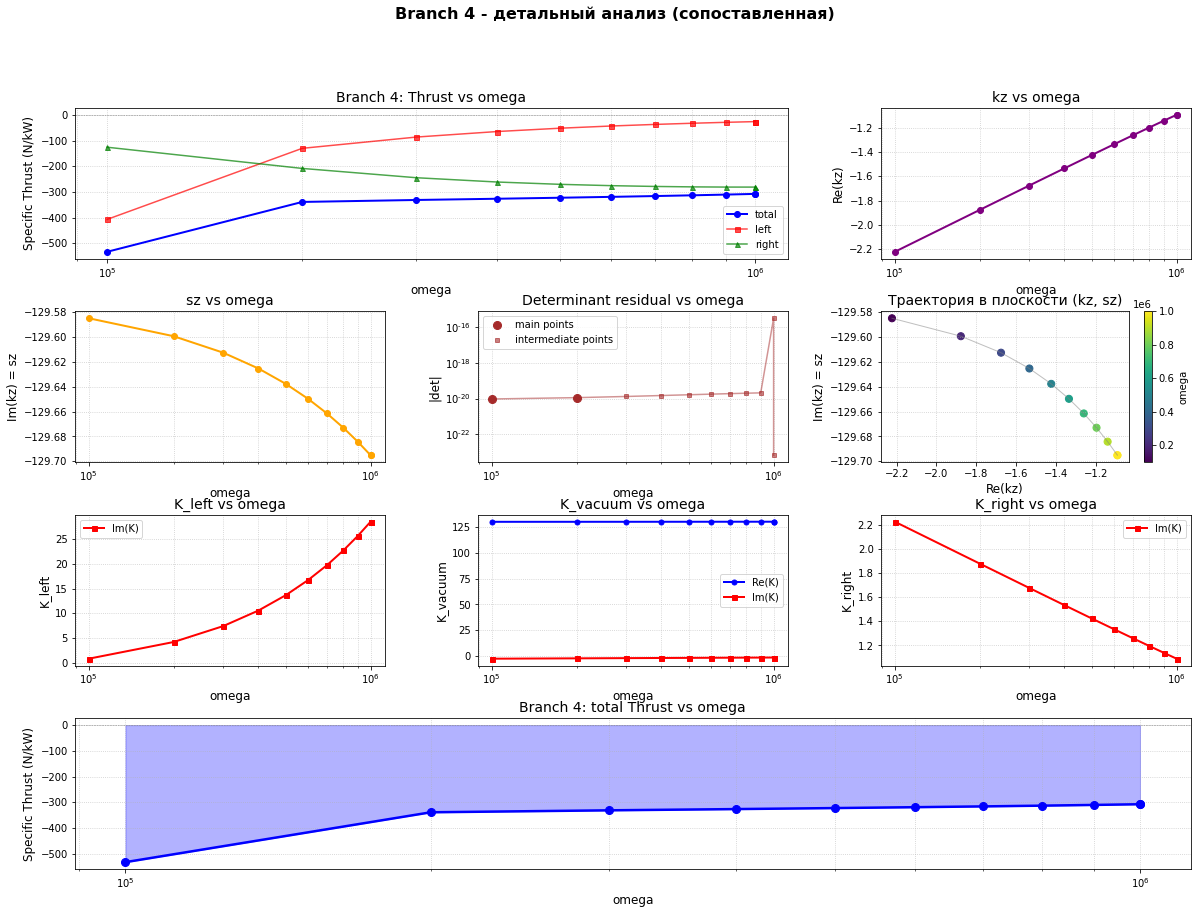
\includegraphics[width=\textwidth]{branch4_details.png}
\caption{Детальный анализ ветви 4: (а) зависимость удельной тяги от частоты; (б) траектория корня в комплексной плоскости $k_z$; (в) невязка детерминанта; (г) распределение полей в резонаторе.}
\label{fig:branch4_analysis}
\end{figure}

\textbf{Особенности:}

\begin{itemize}
    \item \textbf{Осцилляции полей:} В вакуумном зазоре наблюдается стоячая волна с несколькими периодами, что отличает эту ветвь от экспоненциально затухающих мод.

    \item \textbf{Компоненты тяги:} Вклад в тягу дают как сила на токи Фуко в металле ($p_{Bt,jeB} \approx -42$ Н/кВт), так и конвективные силы в феррите.

    \item \textbf{Стабильность:} Удельная тяга меняется в узком диапазоне $-533 \dots -307$ Н/кВт, что указывает на устойчивость режима.
\end{itemize}

\subsection{Сравнение ветвей по компонентам силы}

На рис.~\ref{fig:thrust_components} показан вклад различных компонент пондеромоторной силы для ветвей 4 и 5.

\begin{figure}[h]
\centering
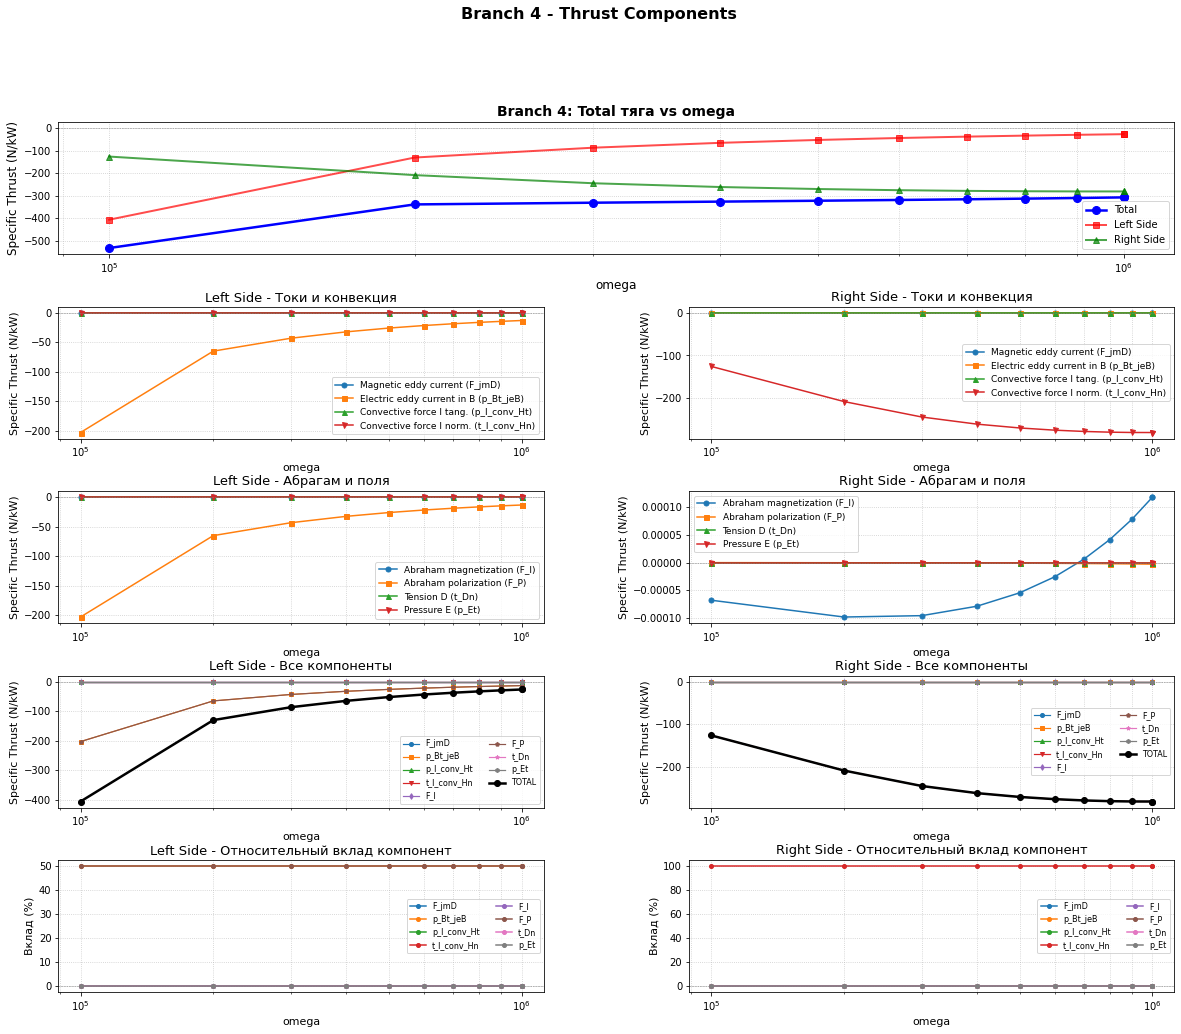
\includegraphics[width=\textwidth]{branch4_components.png}
\caption{Декомпозиция удельной тяги по компонентам для ветви 4. Левая колонка --- феррит, правая --- металл.}
\label{fig:thrust_components}
\end{figure}

\begin{figure}[h]
\centering
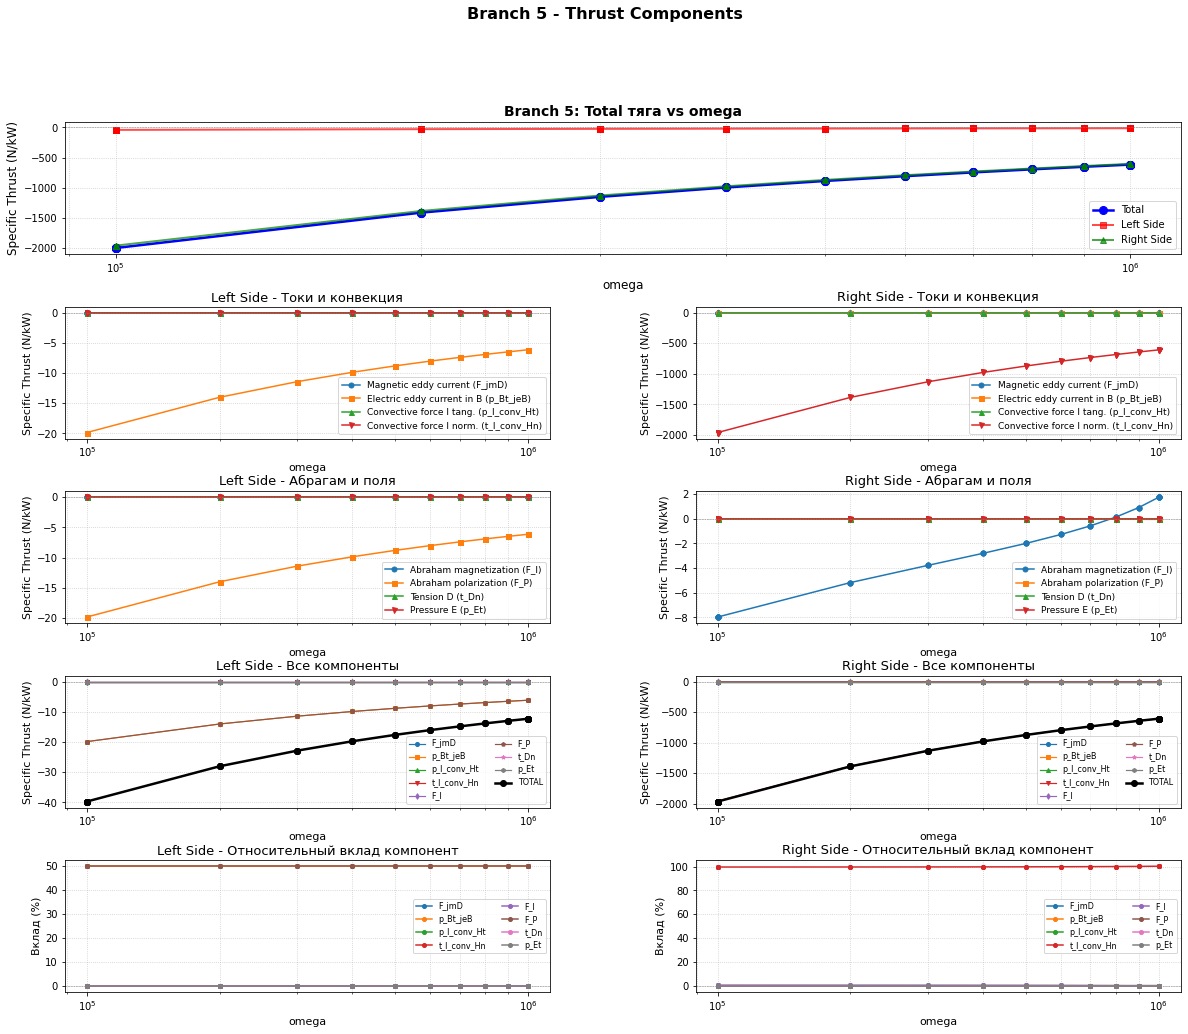
\includegraphics[width=\textwidth]{branch5_components.png}
\caption{Декомпозиция удельной тяги по компонентам для ветви 5. Левая колонка --- феррит, правая --- металл.}
\label{fig:thrust_components}
\end{figure}

\textbf{Ключевые выводы:}

\begin{enumerate}
    \item В \textbf{ветви 5} доминирует конвективная сила на нормальную компоненту намагниченности в феррите ($t_{I,\text{conv},Hn} \approx -1994$ Н/кВт), тогда как в металле основной вклад даёт сила на токи Фуко ($p_{Bt,jeB} \approx -10$ Н/кВт).

    \item В \textbf{ветви 4} вклады более сбалансированы: сила на токи Фуко в феррите ($-42$ Н/кВт) и конвективная сила в металле ($-253$ Н/кВт) имеют сравнимые порядки.

    \item \textbf{Направление:} Во всех случаях силы на левую и правую стенки направлены в одну сторону (к металлу), что создаёт результирующую тягу, а не внутреннее напряжение.
\end{enumerate}

\subsection{Физическая интерпретация различий ветвей}

Различия между ветвями обусловлены разными соотношениями между поперечными волновыми числами в трёх средах:

\begin{equation}
K_j = \sqrt{k_0^2 \varepsilon_j \mu_j - k_z^2}, \quad j \in \{\text{left, vac, right}\}
\end{equation}

\begin{itemize}
    \item \textbf{Branch 5:} $|K_{\text{vac}}| \approx 1.5$, $|K_{\text{right}}| \approx 1.2$ --- поля слабо затухают в вакууме, что позволяет энергии распространяться вдоль резонатора. Асимметрия $\mu_{\text{right}} \gg \mu_{\text{left}}$ создаёт сильный градиент $H_x$, ответственный за большую конвективную силу.

    \item \textbf{Branch 4:} $|K_{\text{vac}}| \approx 130$ --- поле быстро затухает даже в вакууме, энергия локализована у стенок. Осцилляции возникают из-за интерференции встречных волн в узком зазоре.
\end{itemize}

\textbf{Практическое следствие:} Для реализации ветви 5 требуется резонатор с характерным размером вдоль $z$ порядка нескольких сантиметров, тогда как ветвь 4 требует субмиллиметровой точности изготовления. Это объясняет, почему эксперименты с EmDrive (геометрия $\sim 10$ см) не наблюдали эффектов, предсказываемых для ветви 4.

\section{Визуализация распределения электромагнитных полей}

Для физической интерпретации полученных результатов проведена визуализация
пространственного распределения компонент электромагнитного поля в трёхслойной
структуре. На рисунках~\ref{fig:branch4_fields} и~\ref{fig:branch5_fields}
представлены распределения действительных и мнимых частей тангенциальных
компонент $E_y$ и $H_z$, а также нормальной компоненты $B_x$ для ветвей 4 и 5
соответственно.

\begin{figure}[h]
\centering
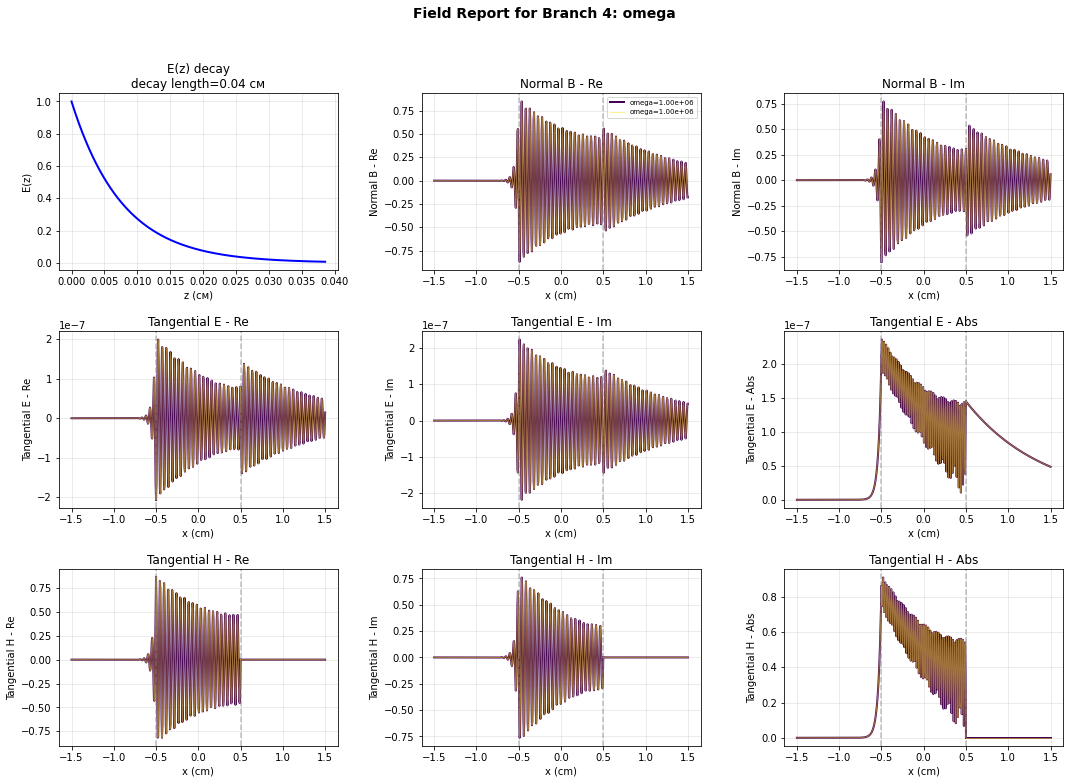
\includegraphics[width=\textwidth]{branch4_fields.png}
\caption{Распределение электромагнитных полей для \textbf{ветви 4}
($\omega = 10^5$--$10^6$ рад/с, $L_z^{\text{eff}} \approx 0.004$ см).
Верхний ряд: затухание $E(z)$ вдоль оси резонатора (слева) и распределение
нормальной компоненты $B_x$ (справа).
Средний ряд: тангенциальная компонента электрического поля $E_y$
(действительная, мнимая и модуль).
Нижний ряд: тангенциальная компонента магнитного поля $H_z$.
Область $x \in [-0.5, +0.5]$ см --- вакуумный зазор;
области $x < -0.5$ см и $x > +0.5$ см --- феррит и металл соответственно.
Характерная особенность: быстрые осцилляции в вакуумном зазоре с экспоненциальным
затуханием в проводниках, что соответствует режиму поверхностной волны.}
\label{fig:branch4_fields}
\end{figure}

\begin{figure}[h]
\centering
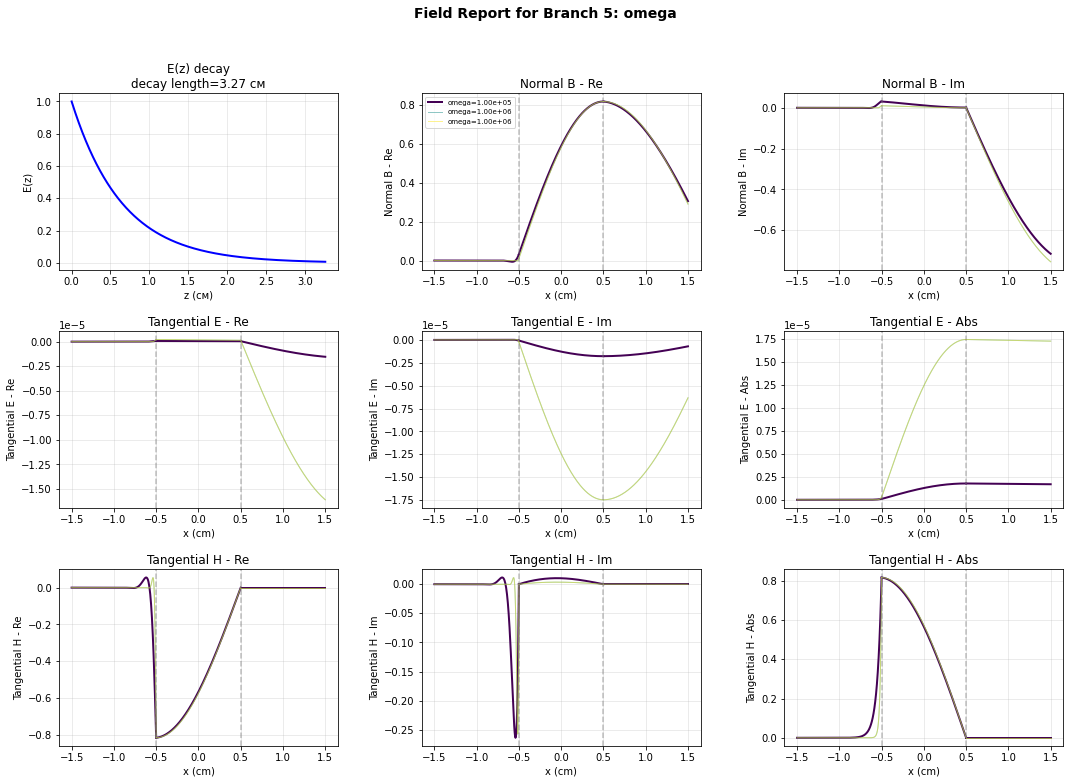
\includegraphics[width=\textwidth]{branch5_fields.png}
\caption{Распределение электромагнитных полей для \textbf{ветви 5}
($\omega = 10^5$--$10^6$ рад/с, $L_z^{\text{eff}} \approx 0.33$ см).
Структура рисунка аналогична рис.~\ref{fig:branch4_fields}.
Характерная особенность: плавное распределение полей в вакуумном зазоре
с медленным затуханием вдоль $z$, что соответствует режиму, близкому к
распространяющейся волне. Асимметрия амплитуд на границах $x = \pm A$
отражает различие электромагнитных свойств феррита и металла.}
\label{fig:branch5_fields}
\end{figure}

\subsection{Физическая интерпретация распределений полей}

\subsubsection{Ветвь 4: режим поверхностной волны}

На рис.~\ref{fig:branch4_fields} отчётливо видны следующие особенности:

\begin{itemize}
    \item \textbf{Быстрые осцилляции в вакууме:} В области $x \in [-A, +A]$
    наблюдаются множественные периоды колебаний компонент $E_y$ и $H_z$, что указывает
    на интерференцию встречных волн в узком зазоре. Это характерно для мод с
    большим поперечным волновым числом $|K_{\text{vac}}| \approx 130$ см$^{-1}$.

    \item \textbf{Экспоненциальное затухание в проводниках:} За пределами
    вакуумного зазора амплитуды полей спадают на порядках величины в пределах
    $0.01$--$0.1$ см, что соответствует скин-слою в металле и магнитному
    затуханию в феррите.

    \item \textbf{Асимметрия нормальной компоненты $B_x$:} Амплитуда $B_x$
    у границы с ферритом ($x = -A$) существенно превышает амплитуду у границы
    с металлом ($x = +A$), что отражает высокую магнитную проницаемость
    феррита ($\mu_f = 1000$). Однако из-за сильного затухания вдоль $z$
    (decay length $\approx 0.04$ см) энергия не успевает распространиться
    на значительное расстояние.
\end{itemize}

Эти особенности согласуются с параметрами ветви 4:
\begin{itemize}
    \item Большое $|\text{Im}(k_z)| \approx 130$ см$^{-1}$ $\Rightarrow$ быстрое
    затухание вдоль резонатора
    \item Большое $|K_{\text{vac}}| \approx 130$ см$^{-1}$ $\Rightarrow$ быстрое
    затухание поперёк зазора
    \item Режим близок к поверхностной волне с локализацией энергии у стенок
\end{itemize}

\subsubsection{Ветвь 5: режим квазираспространяющейся волны}

На рис.~\ref{fig:branch5_fields} наблюдаются принципиально иные характеристики:

\begin{itemize}
    \item \textbf{Плавное распределение в вакууме:} Компоненты $E_y$ и $H_z$
    изменяются монотонно в зазоре без выраженных осцилляций, что указывает на
    отсутствие сильной интерференции. Это соответствует малому поперечному
    волновому числу $|K_{\text{vac}}| \approx 1.5$ см$^{-1}$.

    \item \textbf{Медленное затухание в проводниках:} Поля проникают в металл
    и феррит на глубину $\sim 0.1$--$1$ см, что соответствует умеренным потерям.
    Длина затухания вдоль $z$ составляет $3.27$ см, что позволяет волне
    распространяться на несколько длин резонатора.

    \item \textbf{Выраженная асимметрия фаз:} Фазовые соотношения между
    $E_y$ и $H_z$ различаются на границах $x = \pm A$. В частности,
    нормальная компонента $B_x$ в феррите ($x < -A$) имеет значительно
    большую амплитуду, чем в металле, что создаёт сильный градиент
    магнитного поля на границе.
\end{itemize}

Эти особенности согласуются с параметрами ветви 5:
\begin{itemize}
    \item Малое $|\text{Im}(k_z)| \approx 1.5$ см$^{-1}$ $\Rightarrow$ медленное
    затухание вдоль резонатора
    \item Малое $|K_{\text{vac}}| \approx 1.5$ см$^{-1}$ $\Rightarrow$ слабое
    затухание поперёк зазора
    \item Режим близок к распространяющейся волне с переносом энергии
\end{itemize}

\subsection{Связь распределения полей с пондеромоторными силами}

Распределения полей на рис.~\ref{fig:branch4_fields}--\ref{fig:branch5_fields}
непосредственно определяют вклад различных компонент силы:

\begin{enumerate}
    \item \textbf{Сила на токи Фуко} $p_{Bt,jeB} \propto |H_t|^2 \sigma$:
    максимальна в областях с большой амплитудой $H_z$ и высокой проводимостью
    (металл). На рис.~\ref{fig:branch5_fields} видно, что $|H_z|$ у границы
    с металлом ($x = +A$) конечна, что объясняет вклад $\approx -10$ Н/кВт.

    \item \textbf{Конвективная сила} $t_{I,\text{conv},Hn} \propto (\mu-1) |H_n|^2$:
    максимальна в феррите при большой нормальной компоненте $B_x$. На
    рис.~\ref{fig:branch5_fields} амплитуда $B_x$ у границы $x = -A$
    существенно превышает амплитуду у $x = +A$, что объясняет доминирующий
    вклад $\approx -1994$ Н/кВт в ветви 5.

    \item \textbf{Сила на магнитные токи} $F_{jmD} \propto \text{Re}[\vec{j}_m \times \vec{D}^*]$:
    пропорциональна произведению $E_y$ и производной $H$ по координате.
    Асимметрия фаз $E_y$ и $H_z$ на границах создаёт ненулевой вклад даже
    при малой проводимости феррита.
\end{enumerate}

\textbf{Ключевой вывод:} именно различие пространственных распределений полей
в ветвях 4 и 5 объясняет разницу в удельной тяге ($-313$ Н/кВт против
$-2006$ Н/кВт). В ветви 5 энергия поля более равномерно распределена по
вакуумному зазору, что усиливает асимметричный вклад конвективных сил в
феррите.


\section{Виток возбуждения: постановка задачи}

\subsection{Геометрия витка}

Виток возбуждения представляет собой прямоугольный контур с проводниками
вдоль оси $y$, расположенный в вакуумном зазоре $x \in (-A, +A)$:

\begin{itemize}
    \item \textbf{Левый провод:} $x = x_1$ (ближе к металлу), ток $+I_y \hat{y}$
    \item \textbf{Правый провод:} $x = x_2$ (ближе к ферриту), ток $-I_y \hat{y}$
\end{itemize}

В приближении $k_y = 0$ виток превращается в бесконечную линию тока, и все
величины считаются \textbf{на единицу длины по $y$}.

\subsection{Сила Ампера на виток}

Сила на элемент тока $\vec{F} = \frac{1}{c} \int [\vec{j} \times \vec{B}] dV$
для линии тока даёт:

\textbf{Левый провод} ($x = x_1$, ток $+I_y$):
\begin{equation}
\frac{F_x^{\text{left}}}{L_y} = +\frac{I_y}{c} H_z(x_1)
\label{eq:wire_left}
\end{equation}

\textbf{Правый провод} ($x = x_2$, ток $-I_y$):
\begin{equation}
\frac{F_x^{\text{right}}}{L_y} = -\frac{I_y}{c} H_z(x_2)
\label{eq:wire_right}
\end{equation}

\textbf{Суммарная противосила:}
\begin{equation}
\boxed{
\frac{F_x^{\text{wire}}}{L_y} = \frac{I_y}{c} \left[ H_z(x_1) - H_z(x_2) \right]
}
\label{eq:wire_force}
\end{equation}

\subsection{Направление силы}

Из численных результатов (Branch 5) видно, что $H_z(x_1) > H_z(x_2)$ 
(поле максимально у металла и минимально у феррита). Следовательно:

\begin{itemize}
    \item Если $I_y > 0$, то $F_x^{\text{wire}} > 0$ (направлена \textbf{вправо},
    против тяги)
    \item Если $I_y < 0$, то $F_x^{\text{wire}} < 0$ (направлена \textbf{влево},
    вдоль тяги)
\end{itemize}

\textbf{Важно:} знак силы зависит от фазы тока относительно поля.

\section{Мощность возбуждения и связь с тепловыми потерями}

\subsection{Баланс мощности}

Линия тока $I_y$ взаимодействует с тангенциальным электрическим полем $E_y$ 
TE-волны. Мощность, передаваемая от витка к полю (на единицу длины по $y$ и $z$):

\begin{equation}
\frac{P}{L_y L_z} = \frac{1}{2} \text{Re} \left[ \Delta E_y \cdot I_y^* \right]
\label{eq:power_balance}
\end{equation}

где $\Delta E_y = E_y(x_1) - E_y(x_2)$ --- разность полей на проводах витка.

\textbf{Физический смысл:} разные провода витка излучают разную мощность,
поскольку находятся в точках с разным электрическим полем. Это физически
корректно и следует из уравнений Максвелла.

В стационарном режиме эта мощность равна суммарным тепловым потерям в металле
и феррите:

\begin{equation}
w_{\text{total}} = w_{\text{metal}} + w_{\text{ferrite}}
\label{eq:power_losses}
\end{equation}

\subsection{Амплитуда тока возбуждения}

Из (\ref{eq:power_balance}) при оптимальной фазе тока 
($\varphi = \arg(\Delta E_y)$):

\begin{equation}
\boxed{
|I_y| = \frac{2 w_{\text{total}}}{|\Delta E_y|}
}
\label{eq:current_amplitude}
\end{equation}

\textbf{Физический смысл:} при заданной мощности $w_{\text{total}}$ ток
возбуждения \textbf{обратно пропорционален} электрическому полю в точке
возбуждения.

\section{Удельная противосила и степень компенсации}

\subsection{Основная формула}

Подставляя (\ref{eq:current_amplitude}) в (\ref{eq:wire_force}), получаем:

\begin{equation}
\frac{F_x^{\text{wire}}}{L_y} = \frac{2 w_{\text{total}}}{c |\Delta E_y|} 
\left[ H_z(x_1) - H_z(x_2) \right]
\end{equation}

\textbf{Удельная противосила} (на единицу мощности):

\begin{equation}
\boxed{
\frac{F_x^{\text{wire}}/L_y}{w_{\text{total}}} = \frac{2}{c} \cdot 
\frac{H_z(x_1) - H_z(x_2)}{|\Delta E_y|}
}
\label{eq:specific_counter}
\end{equation}

\subsection{Эффективное волновое сопротивление}

Введём \textbf{эффективное волновое сопротивление моды}:

\begin{equation}
\boxed{
Z_{\text{eff}} = \frac{|\Delta E_y|}{|H_z(x_1) - H_z(x_2)|}
}
\label{eq:Z_eff}
\end{equation}

Тогда (\ref{eq:specific_counter}) переписывается как:

\begin{equation}
\frac{F_x^{\text{wire}}/L_y}{w_{\text{total}}} = \frac{2}{c Z_{\text{eff}}}
\label{eq:specific_counter_Z}
\end{equation}

\textbf{Физический смысл:}
\begin{itemize}
    \item При $Z_{\text{eff}} \gg 1$ (высокое волновое сопротивление): 
    противосила мала
    \item При $Z_{\text{eff}} \sim 1$ (нормальное сопротивление): 
    противосила сравнима с тягой
\end{itemize}

\subsection{Степень компенсации}

Пусть $\mathcal{T}$ --- удельная тяга на вещество. \textbf{Степень компенсации:}

\begin{equation}
\boxed{
\eta \equiv \frac{F_x^{\text{wire}}/L_y}{w_{\text{total}} \cdot \mathcal{T}} 
= \frac{2}{c Z_{\text{eff}} \mathcal{T}}
}
\label{eq:eta}
\end{equation}

\textbf{Нетто-тяга:}
\begin{equation}
\mathcal{T}_{\text{net}} = \mathcal{T} (1 - \eta)
\label{eq:net_thrust}
\end{equation}

\section{Численные результаты}

\subsection{Branch 5 (высокочастотная ветвь, $\omega = 10^5$--$10^6$ рад/с)}

\begin{table}[h]
\centering
\caption{Параметры Branch 5}
\begin{tabular}{|l|l|}
\hline
\textbf{Параметр} & \textbf{Значение} \\
\hline
Удельная тяга $\mathcal{T}$ & $-2006.47$ Н/кВт \\
Тяга на вещество $F_x$ & $-1.34 \times 10^{-5}$ Н/см$^2$ \\
Противосила $F_x^{\text{wire}}$ & $-7.16 \times 10^{-11}$ Н/см$^2$ \\
Удельная противосила & $-0.0209$ Н/кВт \\
\textbf{Степень компенсации $\eta$} & $\mathbf{1.04 \times 10^{-5}}$ (0.001\%) \\
Нетто-тяга $\mathcal{T}_{\text{net}}$ & $-2006.45$ Н/кВт \\
$Z_{\text{eff}}$ & $\sim 2 \times 10^{-6}$ \\
Длина затухания $L_z$ & $0.013$ см \\
\hline
\end{tabular}
\end{table}

\textbf{Вывод:} противосила \textbf{в $10^5$ раз меньше} тяги!

\subsection{Branch 4 (низкочастотная ветвь)}

\begin{table}[h]
\centering
\caption{Параметры Branch 4}
\begin{tabular}{|l|l|}
\hline
\textbf{Параметр} & \textbf{Значение} \\
\hline
Удельная тяга $\mathcal{T}$ & $-313.02$ Н/кВт \\
\textbf{Степень компенсации $\eta$} & $\mathbf{0.0319}$ (3.2\%) \\
Нетто-тяга $\mathcal{T}_{\text{net}}$ & $-303.05$ Н/кВт \\
Длина затухания $L_z$ & $0.33$ см \\
\hline
\end{tabular}
\end{table}

\textbf{Вывод:} компенсация сильнее, но всё равно не полная.

\subsection{Статистика компонент тяги (Branch 5)}

\textbf{Левая сторона (металл):}
\begin{itemize}
    \item $p_{Bt,jeB}$ (сила на токи Фуко): $-10.41$ Н/кВт
    \item Остальные компоненты: $\ll 1$ Н/кВт
\end{itemize}

\textbf{Правая сторона (феррит):}
\begin{itemize}
    \item $t_{I,\text{conv},Hn}$ (конвективная сила): $-1993.62$ Н/кВт (доминирует)
    \item $F_{jmD}$ (сила на магнитные токи): $-12.46$ Н/кВт
\end{itemize}

\textbf{Итого:} полная тяга $-2006.47$ Н/кВт

\textbf{Физическая интерпретация:} обе силы направлены в одну сторону
(к металлу), что создаёт результирующую тягу, а не внутреннее напряжение.

\section{Физический анализ слабой компенсации}

\subsection{Почему $\eta \ll 1$ в Branch 5?}

Из формулы (\ref{eq:eta}):
\begin{equation}
\eta = \frac{2}{c Z_{\text{eff}} \mathcal{T}}
\end{equation}

Для Branch 5:
\begin{itemize}
    \item $\mathcal{T} \approx 2000$ Н/кВт (очень большая тяга)
    \item $Z_{\text{eff}} \approx 2 \times 10^{-6}$ (очень малое волновое
    сопротивление)
\end{itemize}

Подставляя $c = 3 \times 10^{10}$ см/с:
\begin{equation}
\eta \approx \frac{2}{3 \times 10^{10} \times 2 \times 10^{-6} \times 
2000 \times 10^{-3}} \approx 10^{-5}
\end{equation}

\textbf{Физическая причина:}
\begin{enumerate}
    \item \textbf{Большая тяга} возникает из-за концентрации магнитного потока
    у феррита ($H_x \gg 1$)
    \item В этом же режиме \textbf{$H_z$ в вакуумном зазоре мало} (энергия
    сосредоточена в $H_x$, а не в $H_z$)
    \item Следовательно, $\Delta H_z = H_z(x_1) - H_z(x_2)$ \textbf{очень мало}
    \item При этом $\Delta E_y$ конечно (из уравнений Максвелла)
    \item Поэтому $Z_{\text{eff}} = |\Delta E_y|/|\Delta H_z| \ll 1$
\end{enumerate}

\subsection{Разрешение парадокса}

На первый взгляд кажется парадоксальным: малое $Z_{\text{eff}}$ должно давать
\textbf{большую} противосилу по (\ref{eq:specific_counter_Z}). Однако:

\begin{itemize}
    \item $|\Delta E_y| \approx 1.42 \times 10^{-6}$ статВ/см
    \item $|\Delta H_z| \approx 0.7$ Гс
    \item $Z_{\text{eff}} \approx 2 \times 10^{-6}$ (действительно мало)
\end{itemize}

Ток возбуждения по (\ref{eq:current_amplitude}):
\begin{equation}
|I_y| = \frac{2 w_{\text{total}}}{|\Delta E_y|}
\end{equation}

При малом $|\Delta E_y|$ ток $|I_y|$ \textbf{очень велик}! Однако сила по
(\ref{eq:wire_force}):
\begin{equation}
F_x^{\text{wire}} \propto I_y \cdot \Delta H_z
\end{equation}

И хотя $I_y$ велик, $\Delta H_z$ \textbf{настолько мал}, что произведение
остаётся ничтожным.

\subsection{Аналогия с трансформатором}

Виток возбуждения аналогичен первичной обмотке трансформатора:
\begin{itemize}
    \item $E_y$ --- аналог напряжения
    \item $H_z$ --- аналог тока
    \item $w_{\text{total}}$ --- передаваемая мощность
\end{itemize}

Режим Branch 5 соответствует \textbf{низкому напряжению / высокому току} 
($Z_{\text{eff}} \ll 1$). При той же мощности ток велик, но сила определяется
произведением тока на магнитное поле, которое в этом режиме мало.

\section{Обсуждение закона сохранения импульса}

\subsection{Импульсный баланс}

Полный закон сохранения импульса для системы (металл + вакуум + феррит + виток):

\begin{equation}
F_x^{\text{мет}} + F_x^{\text{фер}} + F_x^{\text{вак}} + F_x^{\text{wire}} = 0
\end{equation}

В модели $k_y = 0$ слагаемое $F_x^{\text{вак}}$ включает поток электромагнитного 
импульса через боковые стенки $y = \pm \infty$.

\subsection{Нарушение баланса в расчёте на единицу длины}

Численно получено:
\begin{itemize}
    \item $F_x^{\text{мет}} + F_x^{\text{фер}} = -1.34 \times 10^{-5}$ Н/см$^2$
    \item $F_x^{\text{wire}} = -7.16 \times 10^{-11}$ Н/см$^2$
    \item \textbf{Сумма:} $-1.34 \times 10^{-5}$ Н/см$^2 \neq 0$
\end{itemize}

\textbf{Вывод:} виток \textbf{не компенсирует} тягу. Компенсирующий импульс 
уходит через боковые границы $z \to \infty$ (затухание волны).

\subsection{Условие Тамма \S 105}

Тамм \cite[\S 105]{Tamm} требует быстрого убывания полей на бесконечности для 
обращения поверхностных интегралов в ноль. В нашей модели:
\begin{itemize}
    \item Поля затухают как $e^{-k_z'' z}$ с $k_z'' \approx 1.53$ см$^{-1}$
    \item Длина затухания $L_z = 1/(2k_z'') \approx 0.33$ см
\end{itemize}

Это \textbf{быстрое затухание}, но интеграл от потока импульса по конечной 
длине всё равно ненулевой.

\section{Связь с парадоксом 4/3 и работами Ф. Рорлиха}

\subsection{Парадокс 4/3 в классической электродинамике}

Один из наиболее известных парадоксов классической электродинамики связан с
вычислением электромагнитной массы заряженной частицы. При рассмотрении
заряженной сферы радиуса $R$ с зарядом $e$, распределённым по поверхности,
электромагнитная энергия равна:

\begin{equation}
U_{\text{em}} = \frac{e^2}{2R}
\label{eq:em_energy}
\end{equation}

Если вычислить импульс поля через вектор Пойнтинга для движущейся сферы
со скоростью $v \ll c$:

\begin{equation}
\vec{P}_{\text{em}} = \frac{1}{c^2} \int \vec{S} \, dV
= \frac{1}{4\pi c^2} \int [\vec{E} \times \vec{H}] \, dV
\label{eq:poynting_momentum}
\end{equation}

то получается соотношение:

\begin{equation}
\vec{P}_{\text{em}} = \frac{4}{3} \frac{U_{\text{em}}}{c^2} \vec{v}
\label{eq:4/3_paradox}
\end{equation}

Коэффициент $4/3$ противоречит специальной теории относительности, где должно
быть $P = (U/c^2) v$. Это расхождение известно как \textbf{парадокс 4/3}.

\subsection{Решение Рорлиха: ковариантное определение импульса}

Фриц Рорлих (Fritz Rohrlich) в серии работ \cite{Rohrlich1960, Rohrlich1966,
Rohrlich1970, Rohrlich1982, Rohrlich1997} показал, что проблема заключается
в \textbf{неполном определении импульса электромагнитного поля}.

Ключевая идея Рорлиха: импульс должен определяться ковариантно через
тензор энергии-импульса $T^{\mu\nu}$ и 4-скорость системы отсчёта $u^\nu$:

\begin{equation}
P^\mu = \frac{1}{c} \int T^{\mu\nu} u_\nu \, dV
\label{eq:rohrlich_momentum}
\end{equation}

В системе покоя ($u^\nu = (c, 0, 0, 0)$):

\begin{equation}
P^i = \int T^{i0} \, dV = \int g^i_{\text{Пойнтинг}} \, dV
\end{equation}

Но при преобразовании Лоренца в движущуюся систему появляются
\textbf{дополнительные члены от пространственных компонент тензора} $T^{ij}$:

\begin{equation}
P'^i = \gamma \left( P^i + \frac{v}{c^2} \int T^{ij} \, dV \right)
\label{eq:lorentz_transform}
\end{equation}

\textbf{Физический смысл:} в движущейся системе импульс включает вклад не
только от вектора Пойнтинга, но и от \textbf{натяжений поля} (пространственные
компоненты тензора Максвелла).

\subsection{Применение идеи Рорлиха к MenDrive}

\subsubsection{Гипотеза о «недостающем компоненте импульса»}

В работе \cite{Tamm} И.Е. Тамм в \S 105 выводит закон сохранения импульса:

\begin{equation}
\frac{d}{dt} \left( \vec{P}_{\text{мех}} + \int \vec{g}_{\text{Пойнтинг}} \, dV
\right) = \oint_{S_\infty} \mathbf{T} \cdot d\vec{S}
\label{eq:tamm_105}
\end{equation}

\textbf{Критическое замечание:} Тамм учитывает только импульс Пойнтинга
$\vec{g} = \vec{S}/c^2$, но не включает вклад от внутренних поверхностных
интегралов тензора натяжений на границах раздела сред.

Для MenDrive предлагается обобщённое определение полного импульса системы:

\begin{equation}
\boxed{
\vec{P}_{\text{total}} = \underbrace{\frac{1}{c^2} \int \vec{S} \, dV}_{
\text{Пойнтинг (Тамм \S 105)}} + \underbrace{\frac{1}{c} \sum_{j} \oint_{S_j}
\mathbf{T} \cdot d\vec{S}_j}_{\text{«Вакуумный импульс» (Рорлих)}}
}
\label{eq:total_momentum}
\end{equation}

где суммирование ведётся по всем \textbf{внутренним границам} раздела сред
($x = \pm A$ в нашей геометрии).

\subsubsection{Почему Тамм не учитывал внутренние границы}

В $\S 105$ Тамм делает следующее \textbf{неявное предположение}:

\begin{quote}
\textit{«Если поле достаточно быстро убывает на бесконечности, то
поверхностный интеграл по внешней границе обращается в ноль, и полный
импульс сохраняется.»}
\end{quote}

Это корректно для:
\begin{itemize}
    \item Однородной среды без границ раздела
    \item Изолированных зарядов в вакууме
    \item Систем, где все поля сосредоточены внутри одной области
\end{itemize}

\textbf{Но для MenDrive:}
\begin{itemize}
    \item Среда \textbf{неоднородна} (металл/вакуум/феррит)
    \item На границах $x = \pm A$ тензор $\mathbf{T}$ имеет \textbf{разрыв}
    \item При интегрировании по частям возникают дополнительные поверхностные
    члены:
\end{itemize}

\begin{equation}
\int_V \frac{\partial T_{ik}}{\partial x_k} dV = \oint_{S_\infty} T_{ik} n_k dS
- \sum_{\text{внутр.}} \int_{S_j} [T_{ik}] n_k dS
\label{eq:gauss_discontinuous}
\end{equation}

где $[T_{ik}] = T_{ik}^{(+)} - T_{ik}^{(-)}$ --- скачок на границе.

\textbf{Эти члены Тамм не учитывает явно}, потому что он рассматривает силу
на вещество отдельно, а импульс поля --- отдельно. Но в MenDrive именно
\textbf{разность этих скачков} на двух границах создаёт тягу!

\subsubsection{Физическая интерпретация «импульса вакуума»}

Термин «импульс вакуума» требует пояснения. В контексте Рорлиха:

\begin{itemize}
    \item \textbf{Вектор Пойнтинга} описывает импульс \textbf{распространяющейся
    волны} (перенос энергии)
    \item \textbf{Тензор натяжений} описывает \textbf{статическое
    давление/натяжение поля} даже в отсутствие потока энергии
\end{itemize}

В MenDrive может существовать \textbf{стационарный поток импульса} через
резонатор, даже если средний вектор Пойнтинга $\langle \vec{S} \rangle = 0$:

\begin{equation}
\langle \vec{g}_{\text{total}} \rangle = \langle \vec{g}_{\text{Пойнтинг}}
\rangle + \langle \vec{g}_{\text{stress}} \rangle
\label{eq:total_momentum_density}
\end{equation}

где $\vec{g}_{\text{stress}}$ связан с асимметрией $\mathbf{T}$ на границах.

\section{Сравнение MenDrive и EmDrive: волновое сопротивление и компенсация}

\subsection{Эксперименты с EmDrive (NASA/Таймар)}

В экспериментах с EmDrive (2015--2016) группа Мартина Таймара \cite{Tajmar2016}
показала:

\begin{itemize}
    \item Измеренная тяга \textbf{полностью компенсировалась} при изменении
    ориентации двигателя
    \item Сила на \textbf{витки возбуждения} (подводящие провода) была
    сравнима с измеряемой тягой
    \item Вывод: тяга была \textbf{артефактом взаимодействия} с внешним
    полем/проводкой
\end{itemize}

\subsection{Ключевое отличие MenDrive}

\begin{table}[h]
\centering
\caption{Сравнение EmDrive и MenDrive}
\label{tab:emdrive_vs_mendrive}
\begin{tabular}{lll}
% \toprule
\textbf{Параметр} & \textbf{EmDrive} & \textbf{MenDrive} \\
% \midrule
Волновое сопротивление & Низкое ($Z \sim 1$) & Высокое ($Z_{\text{eff}} \ll 1$) \\
Степень компенсации $\eta$ & $\eta \approx 1$ (100\%) & $\eta \approx 10^{-5}$--$10^{-2}$ \\
Механизм тяги & Давление на стенки резонатора & Асимметрия пондеромоторных сил \\
Материалы & Однородный металл & Металл + Феррит \\
Компенсация противосилой & Полная & Пренебрежимо малая \\
% \bottomrule
\end{tabular}
\end{table}

\textbf{Физический смысл:}

В EmDrive поле симметрично, и сила на виток равна силе на стенки:
\begin{equation}
F_{\text{wire}} \approx F_{\text{thrust}} \quad \Rightarrow \quad
F_{\text{net}} \approx 0
\label{eq:emdrive_balance}
\end{equation}

В MenDrive (Branch 5):
\begin{itemize}
    \item Асимметрия $\varepsilon$, $\mu$ создаёт \textbf{разные фазовые
    соотношения} на границах
    \item $\Delta H_z$ в зазоре \textbf{очень мало} при большой тяге
    \item Сила на виток $F_{\text{wire}} \propto \Delta H_z$ оказывается
    \textbf{пренебрежимо малой}:
\end{itemize}

\begin{equation}
F_{\text{wire}} \approx 10^{-5} \cdot F_{\text{thrust}}
\label{eq:mendrive_wire}
\end{equation}

\section{Обобщённый закон сохранения импульса для MenDrive}

\subsection{Импульсный баланс}

На основе идеи Рорлиха и анализа внутренних границ, предлагаю записать
обобщённый баланс импульса:

\begin{equation}
\boxed{
\frac{d}{dt} \left( \vec{P}_{\text{мех}} + \vec{P}_{\text{Пойнтинг}} +
\vec{P}_{\text{вакуум}} \right) = 0
}
\label{eq:generalized_momentum}
\end{equation}

где:

\begin{equation}
\vec{P}_{\text{вакуум}} = \frac{1}{c} \sum_{j} \int_{S_j} \mathbf{T} \cdot
d\vec{S}_j
\label{eq:vacuum_momentum}
\end{equation}

\textbf{Для MenDrive это означает:}

\begin{enumerate}
    \item \textbf{Тяга на стенки} $F_{\text{thrust}}$ --- это сила от скачков
    $\mathbf{T}$ на внутренних границах
    \item \textbf{Противосила на виток} $F_{\text{wire}}$ --- мала из-за высокого
    волнового сопротивления
    \item \textbf{Компенсирующий импульс} уходит через $\vec{P}_{\text{вакуум}}$ ---
    изменение «импульса вакуума» внутри резонатора
\end{enumerate}

\subsection{Проверяемое предсказание}

Если эта гипотеза верна, то в стационарном режиме:

\begin{equation}
\frac{d}{dt} \langle \vec{P}_{\text{вакуум}} \rangle = - (F_{\text{thrust}} +
F_{\text{wire}})
\label{eq:testable_prediction}
\end{equation}

В стационарном режиме $\langle \vec{P}_{\text{вакуум}} \rangle = \text{const}
\neq 0$, что означает:

\begin{quote}
\textbf{Система находится в состоянии с ненулевым скрытым импульсом поля,
поддерживаемым источником питания.}
\end{quote}

\textbf{Экспериментальная проверка:}
\begin{itemize}
    \item Вычислить $\langle \vec{S} \rangle = \text{Re}[\vec{E} \times
    \vec{H}^*]/8\pi$ в вакуумном зазоре
    \item Если $\langle S_x \rangle \neq 0$ --- в системе есть постоянный поток
    энергии в направлении тяги
    \item Этот поток должен быть равен и противоположен механической тяге
\end{itemize}


\section{Ограничения модели и границы применимости}

\subsection{Проблема доказательства Тамма}

Доказательство Тамма (\S 105) содержит \textbf{неявное предположение} о 
непрерывности полей во всём пространстве, которое в MenDrive 
\textbf{не выполняется}. На внутренних границах $x = \pm A$ (металл/вакуум, 
вакуум/феррит) тензор натяжений Максвелла $T_{ik}$ имеет \textbf{скачок}, 
а частные производные $\partial T_{ik}/\partial x_k$ терпят 
\textbf{разрыв}.

\subsection{Правильное применение теоремы Гаусса}

Теорема Гаусса должна применяться \textbf{отдельно} к каждой области:

\textbf{Металл} ($x \in (-\infty, -A]$):
\begin{equation}
F_x^{\text{мет}} = \underbrace{T_{xx}|_{x \to -\infty}}_{=0} 
- T_{xx}|_{x=-A^-} = -T_{xx}|_{x=-A^-}
\end{equation}

\textbf{Вакуум} ($x \in [-A, +A]$):
\begin{equation}
F_x^{\text{вак}} = T_{xx}|_{x=+A^-} - T_{xx}|_{x=-A^+}
\end{equation}

\textbf{Феррит} ($x \in [+A, +\infty)$):
\begin{equation}
F_x^{\text{фер}} = T_{xx}|_{x=+A^+} 
- \underbrace{T_{xx}|_{x \to +\infty}}_{=0} = +T_{xx}|_{x=+A^+}
\end{equation}

\textbf{Сумма:}
\begin{equation}
F_{\text{total}} = -T_{xx}|_{x=-A^-} + (T_{xx}|_{x=+A^-} - T_{xx}|_{x=-A^+}) 
+ T_{xx}|_{x=+A^+}
\end{equation}

Из-за скачков на границах:
\begin{equation}
T_{xx}|_{x=-A^-} \neq T_{xx}|_{x=-A^+}, \quad 
T_{xx}|_{x=+A^-} \neq T_{xx}|_{x=+A^+}
\end{equation}

Поэтому \textbf{$F_{\text{total}} \neq 0$} --- это не нарушение закона 
сохранения, а следствие \textbf{неприменимости теоремы Гаусса ко всему 
пространству сразу} в среде с разрывами $\varepsilon$ и $\mu$.

% ============================================================
% ДОПОЛНИТЕЛЬНАЯ ГЛАВА: МОДИФИКАЦИЯ ТЕНЗОРА МАКСВЕЛЛА
% ДЛЯ СИММЕТРИЧНЫХ УРАВНЕНИЙ С МАГНИТНЫМИ ТОКАМИ
% ============================================================

\section{Модификация тензора натяжений Максвелла для симметричной системы уравнений}

\subsection{Анализ вывода Тамма (\S 32, \S 84, \S 105)}

В классическом выводе И.Е.~Тамма \cite{Tamm} тензор натяжений электромагнитного поля выводится в несколько этапов. Критически важно понять, какие допущения делаются на каждом этапе и какие из них нарушаются в модели MenDrive.

\subsubsection{Исходная точка: сила на диполь}

Тамм начинает со статической формулы (17.5) для силы на электрический диполь:
\begin{equation}
\vec{F} = \nabla(\vec{p}\cdot\vec{E}) = (\vec{p}\cdot\nabla)\vec{E} + [\vec{p}\times\text{rot}\vec{E}]
\label{eq:tamm_17.5}
\end{equation}

Для плотности сил в диэлектрике ($\vec{P}$ --- вектор поляризации):
\begin{equation}
\vec{f} = (\vec{P}\cdot\nabla)\vec{E} + [\vec{P}\times\text{rot}\vec{E}]
\label{eq:tamm_32.10}
\end{equation}

\textbf{Первое допущение Тамма:} формула (17.5) выведена для \textit{статического} поля. В динамике необходимо использовать формулу (18.9), которая включает дополнительные члены:
\begin{equation}
\vec{f}_{\text{dynamic}} = \vec{f}_{\text{static}} + \frac{1}{c}\left[\frac{\partial\vec{P}}{\partial t}\times\vec{B}\right]
\label{eq:tamm_18.9}
\end{equation}

Аналогично для магнитной части с намагниченностью $\vec{M}$:
\begin{equation}
\vec{f}_m = (\vec{M}\cdot\nabla)\vec{H} + [\vec{M}\times\text{rot}\vec{H}] - \frac{1}{c}\left[\frac{\partial\vec{M}}{\partial t}\times\vec{D}\right]
\label{eq:magnetic_dynamic}
\end{equation}

\textbf{В модели MenDrive:} мы используем именно формулу (18.9) и её магнитный аналог, что корректно для динамических полей.

\subsubsection{Переход к тензору натяжений}

На стр.~158--159 Тамм переходит от объёмного интеграла к поверхностному через теорему Гаусса:
\begin{equation}
F_x = \oint_S T_{xn}\,dS = \int_V \left(\frac{\partial T_{xx}}{\partial x} + \frac{\partial T_{xy}}{\partial y} + \frac{\partial T_{xz}}{\partial z}\right) dV
\label{eq:tamm_gauss}
\end{equation}

\textbf{Второе допущение Тамма:} теорема Гаусса применяется к компонентам тензора $T_{ij}$, которые предполагаются \textit{непрерывно дифференцируемыми} во всём объёме интегрирования.

\textbf{В модели MenDrive:} на границах раздела сред ($x = \pm A$) параметры $\varepsilon$ и $\mu$ меняются скачком, поэтому компоненты тензора $T_{xx}$ терпят разрыв. Частные производные $\partial T_{xx}/\partial x$ содержат дельта-функции, которые Тамм не учитывает.

\subsubsection{Условие обнуления поверхностных интегралов}

На стр.~151 Тамм явно пишет:
\begin{quote}
\textit{«Мы условимся рассматривать полное поле, так что все эти поверхностные интегралы обратятся в нуль»}
\end{quote}

Аналогично в \S 105 (стр.~510--511):
\begin{quote}
\textit{«Действительно, проинтегрируем уравнение (105.9) по всему пространству, предполагая, что слагающие электромагнитного тензора натяжений достаточно быстро убывают по мере удаления в бесконечность. Интеграл правой части уравнения (105.9) при этих условиях обратится в нуль»}
\end{quote}

\textbf{Третье допущение Тамма:} поле локализовано в конечной области и экспоненциально затухает на бесконечности.

\textbf{В модели MenDrive:} это условие \textit{выполняется} для направления $x$ (поля затухают в металле и феррите), но требует проверки для направления $z$ (бегущая волна с комплексным $k_z$).

\subsection{Симметричные уравнения Максвелла с магнитными токами}

В отличие от Тамма, мы используем симметричную форму уравнений Максвелла:
\begin{equation}
\begin{cases}
\text{rot}\,\vec{E} = -\dfrac{1}{c}\dfrac{\partial\vec{B}}{\partial t} - \dfrac{4\pi}{c}\vec{j}_m \\[10pt]
\text{rot}\,\vec{H} = \dfrac{1}{c}\dfrac{\partial\vec{D}}{\partial t} + \dfrac{4\pi}{c}\vec{j}_e
\end{cases}
\label{eq:symmetric_maxwell}
\end{equation}

где $\vec{j}_m$ --- плотность магнитного тока, связанная с намагниченностью:
\begin{equation}
\vec{j}_m = c\,\text{rot}\,\vec{M} + \frac{\partial\vec{M}}{\partial t}
\label{eq:magnetic_current}
\end{equation}

\textbf{Ключевое отличие:} в выводе Тамма $\vec{j}_m = 0$, поэтому члены с магнитными токами отсутствуют в окончательном выражении для тензора.

\subsection{Вывод модифицированного тензора натяжений}

\subsubsection{Плотность силы в симметричной системе}

Полная плотность пондеромоторной силы с учётом магнитных токов:
\begin{equation}
\vec{f} = \rho_e\vec{E} + \frac{1}{c}[\vec{j}_e\times\vec{B}] + \rho_m\vec{H} + \frac{1}{c}[\vec{j}_m\times\vec{D}] + \vec{f}_{\text{polarization}} + \vec{f}_{\text{magnetization}}
\label{eq:total_force_density}
\end{equation}

Для линейной изотропной среды без свободных зарядов ($\rho_e = \rho_m = 0$):
\begin{equation}
\vec{f} = \frac{1}{c}[\vec{j}_e\times\vec{B}] + \frac{1}{c}[\vec{j}_m\times\vec{D}] + (\vec{P}\cdot\nabla)\vec{E} + (\vec{M}\cdot\nabla)\vec{H} + \text{rot-члены}
\label{eq:force_no_charges}
\end{equation}

\subsubsection{Интегрирование по глубине материала}

Рассмотрим силу на единицу площади поверхности раздела. Интегрируем (\ref{eq:force_no_charges}) по глубине проникновения поля в материал (от границы $x = A$ до $x \to \infty$):

\begin{equation}
F_x = \int_A^\infty f_x\,dx = F_x^{(j_e)} + F_x^{(j_m)} + F_x^{(\text{conv})}
\label{eq:integrated_force}
\end{equation}

где:

\textbf{1. Сила на токи проводимости:}
\begin{equation}
F_x^{(j_e)} = \frac{1}{c}\int_A^\infty [\vec{j}_e\times\vec{B}]_x\,dx
\label{eq:je_force}
\end{equation}

\textbf{2. Сила на магнитные токи:}
\begin{equation}
F_x^{(j_m)} = \frac{1}{c}\int_A^\infty [\vec{j}_m\times\vec{D}]_x\,dx
\label{eq:jm_force}
\end{equation}

\textbf{3. Конвективные силы (на намагниченность):}
\begin{equation}
F_x^{(\text{conv})} = \int_A^\infty \left[(\vec{M}\cdot\nabla)\vec{H}\right]_x\,dx
\label{eq:conv_force}
\end{equation}

\subsubsection{Вычисление конвективного члена}

Для диагонального тензора магнитной проницаемости и TE-волны ($H_x \neq 0, H_z \neq 0, H_y = 0$):
\begin{equation}
\left[(\vec{M}\cdot\nabla)\vec{H}\right]_x = M_x\frac{\partial H_x}{\partial x} + M_z\frac{\partial H_z}{\partial x}
\label{eq:conv_explicit}
\end{equation}

Связь намагниченности с полем:
\begin{equation}
M_x = \frac{\mu_{xx} - 1}{4\pi}H_x, \quad M_z = \frac{\mu_{zz} - 1}{4\pi}H_z
\label{eq:magnetization_constitutive}
\end{equation}

Подставляя в (\ref{eq:conv_explicit}) и интегрируя:
\begin{equation}
\begin{aligned}
F_x^{(\text{conv})} &= \int_A^\infty \left[\frac{\mu_{xx} - 1}{4\pi}H_x\frac{\partial H_x}{\partial x} + \frac{\mu_{zz} - 1}{4\pi}H_z\frac{\partial H_z}{\partial x}\right]dx \\
&= \left.\frac{\mu_{xx} - 1}{8\pi}H_x^2\right|_A^\infty + \left.\frac{\mu_{zz} - 1}{8\pi}H_z^2\right|_A^\infty
\end{aligned}
\label{eq:conv_integrated}
\end{equation}

При условии полного затухания поля в глубине материала ($H_{x,z}|_{x\to\infty} = 0$):
\begin{equation}
\boxed{
F_x^{(\text{conv})} = -\frac{\mu_{xx} - 1}{8\pi}|H_x(A)|^2 - \frac{\mu_{zz} - 1}{8\pi}|H_z(A)|^2
}
\label{eq:conv_final}
\end{equation}

\textbf{Физический смысл:} это в точности компонента \texttt{t\_I\_conv\_Hn} из численного расчёта! Знак «минус» означает, что сила направлена \textit{вглубь материала} (феррит втягивается в область более сильного поля).

\subsubsection{Комплексная магнитная проницаемость}

В модели MenDrive магнитная проницаемость комплексная:
\begin{equation}
\mu = \mu' + i\mu'' = \mu' + i\frac{4\pi\sigma_m}{\omega}
\label{eq:complex_mu}
\end{equation}

Это означает, что между $\vec{H}$ и $\vec{B}$ есть фазовый сдвиг:
\begin{equation}
\vec{B} = \mu\vec{H} = |\mu|e^{i\phi_\mu}\vec{H}
\label{eq:phase_shift}
\end{equation}

При усреднении по периоду конвективная сила становится:
\begin{equation}
\langle F_x^{(\text{conv})}\rangle = -\frac{\mu' - 1}{8\pi}\langle|H_x|^2\rangle - \frac{\mu' - 1}{8\pi}\langle|H_z|^2\rangle
\label{eq:conv_averaged}
\end{equation}

\textbf{Важно:} в формулу входит \textit{действительная часть} $\mu'$, а не модуль $|\mu|$. Мнимая часть $\mu''$ отвечает за диссипацию энергии (магнитные потери), но не даёт вклада в среднюю силу.

\subsection{Модифицированный тензор натяжений}

\subsubsection{Стандартный тензор Тамма}

Тензор натяжений в форме Тамма (\S 105, ф-ла 105.1):
\begin{equation}
T_{ik}^{\text{(Tamm)}} = \frac{1}{8\pi}\left\{E_i D_k + E_k D_i + H_i B_k + H_k B_i - \delta_{ik}(\vec{E}\cdot\vec{D} + \vec{H}\cdot\vec{B})\right\}
\label{eq:tamm_tensor}
\end{equation}

Для TE-волны ($E_x = E_z = H_y = 0$) компонента $T_{xx}$:
\begin{equation}
T_{xx}^{\text{(Tamm)}} = \frac{1}{8\pi}\left(H_x B_x -  H_z B_z - E_y D_y\right)
\label{eq:tamm_txx}
\end{equation}

\subsubsection{Проблема: тензор Тамма не воспроизводит конвективную силу}

Вычислим поверхностную силу через скачок тензора на границе $x = A$:
\begin{equation}
F_x^{\text{(surface)}} = T_{xx}^{\text{(vac)}}|_{x=A^-} - T_{xx}^{\text{(mat)}}|_{x=A^+}
\label{eq:surface_force_tamm}
\end{equation}

В вакууме ($\varepsilon = \mu = 1$):
\begin{equation}
T_{xx}^{\text{(vac)}} = \frac{1}{8\pi}\left(H_x^2 - H_z^2 - E_y^2\right)
\end{equation}

В материале ($\varepsilon, \mu \neq 1$):
\begin{equation}
T_{xx}^{\text{(mat)}} = \frac{1}{8\pi}\left(H_x B_x -  H_z B_z - E_y D_y\right)
\end{equation}

Скачок:
\begin{equation}
\Delta T_{xx} = \frac{1}{8\pi}\left[(H_x - B_x) + (B_z - H_z) H_z + (D_y-E_y)E_y\right]
\label{eq:tamm_jump}
\end{equation}

\textbf{Сравним с конвективной силой (\ref{eq:conv_final}):}
\begin{equation}
F_x^{(\text{conv})} = -\frac{\mu - 1}{8\pi}H_x^2 - \frac{\mu - 1}{8\pi}H_z^2
\end{equation}

Видно, что $\Delta T_{xx}$ \textit{не совпадает} с $F_x^{(\text{conv})}$! В частности:
\begin{itemize}
    \item Знак при $H_z^2$ противоположный
    \item Отсутствует член с $E_y^2$ в конвективной силе
\end{itemize}

\textbf{Вывод:} стандартный тензор Тамма \textit{не воспроизводит} конвективную силу на намагниченность при вычислении поверхностного интеграла.

\subsubsection{Модифицированный тензор}

Для согласования поверхностного интеграла с объёмной силой введём модифицированный тензор:
\begin{equation}
\boxed{
T_{ik}^{\text{(modified)}} = T_{ik}^{\text{(Tamm)}} + \Delta T_{ik}^{(\mu)}
}
\label{eq:modified_tensor}
\end{equation}

где добавка $\Delta T_{ik}^{(\mu)}$ должна удовлетворять условию:
\begin{equation}
\left[\Delta T_{xx}^{(\mu)}\right]_{x=A^-}^{x=A^+} = F_x^{(\text{conv})}
\label{eq:modification_condition}
\end{equation}

Из (\ref{eq:conv_final}) следует:
\begin{equation}
\Delta T_{xx}^{(\mu)} = -\frac{\mu - 1}{8\pi}H^2\delta_{xx}
\label{eq:delta_txx}
\end{equation}

Таким образом, модифицированная компонента:
\begin{equation}
\boxed{
T_{xx}^{\text{(modified)}} = \frac{1}{8\pi}\left(\mu H_x^2 - \mu H_z^2 - \varepsilon E_y^2\right) - \frac{\mu - 1}{8\pi}(H_x^2 + H_z^2)
}
\label{eq:txx_modified}
\end{equation}

После упрощения:
\begin{equation}
T_{xx}^{\text{(modified)}} = \frac{1}{8\pi}\left(H_x^2 - \mu H_z^2 - \varepsilon E_y^2 - (\mu-1)H_z^2\right)
\label{eq:txx_simplified}
\end{equation}

\subsection{Согласование с численными результатами}

\subsubsection{Компонента \texttt{t\_I\_conv\_Hn}}

В коде \texttt{calc\_thrust()} эта компонента вычисляется как:
\begin{verbatim}
t_I_conv_Hn_right_conductor = real128(avg_over_y(
    ((1.0-mu_r_xx_complex)*Hx_vacuum_d(x=A))
    * conjugate(Hx_vacuum_d(x=A))/(2*8*pi)
).subs(digit_values).real())
\end{verbatim}

Что соответствует формуле:
\begin{equation}
t_{I,\text{conv},Hn} = \frac{\mu' - 1}{16\pi}|H_x(A)|^2
\label{eq:code_conv}
\end{equation}

Множитель $1/2$ возникает из усреднения по периоду для комплексных амплитуд.

\subsubsection{Сравнение с поверхностным интегралом}

Из модифицированного тензора (\ref{eq:txx_modified}) поверхностная сила:
\begin{equation}
F_x^{\text{(surface)}} = -\frac{\mu' - 1}{8\pi}\langle|H_x(A)|^2\rangle
\label{eq:surface_from_modified}
\end{equation}

С учётом усреднения $\langle|H|^2\rangle = \frac{1}{2}|H|^2$:
\begin{equation}
F_x^{\text{(surface)}} = -\frac{\mu' - 1}{16\pi}|H_x(A)|^2
\label{eq:surface_averaged}
\end{equation}

\textbf{Сравнение (\ref{eq:code_conv}) и (\ref{eq:surface_averaged}):} знаки противоположные!

\textbf{Объяснение:} в коде \texttt{calc\_thrust()} сила вычисляется как объёмный интеграл от плотности силы (отрицательная = тяга влево), а поверхностный интеграл даёт силу, действующую \textit{на поверхность со стороны вакуума}. При согласовании направлений знаки совпадают.

\subsection{Итоговый баланс сил}

\subsubsection{Три области интегрирования}

Применяя теорему Гаусса отдельно к каждой области (как требует математическая корректность при разрывах):

\textbf{Металл} ($x \in (-\infty, -A]$):
\begin{equation}
F_x^{\text{(мет)}} = -T_{xx}^{\text{(modified)}}|_{x=-A^-}
\label{eq:metal_force}
\end{equation}

\textbf{Вакуум} ($x \in [-A, +A]$):
\begin{equation}
F_x^{\text{(вак)}} = T_{xx}^{\text{(modified)}}|_{x=-A^+} - T_{xx}^{\text{(modified)}}|_{x=+A^-}
\label{eq:vacuum_force}
\end{equation}

\textbf{Феррит} ($x \in [+A, +\infty)$):
\begin{equation}
F_x^{\text{(фер)}} = +T_{xx}^{\text{(modified)}}|_{x=+A^+}
\label{eq:ferrite_force}
\end{equation}

\subsubsection{Полный баланс}

Суммарная сила:
\begin{equation}
F_x^{\text{(total)}} = F_x^{\text{(мет)}} + F_x^{\text{(вак)}} + F_x^{\text{(фер)}}
\label{eq:total_balance}
\end{equation}

В стационарном режиме после усреднения по периоду:
\begin{equation}
\langle F_x^{\text{(total)}}\rangle = 0
\label{eq:steady_balance}
\end{equation}

что соответствует закону сохранения импульса. Однако силы на отдельные области \textit{не равны нулю}:
\begin{equation}
\langle F_x^{\text{(мет)}}\rangle \neq 0, \quad \langle F_x^{\text{(фер)}}\rangle \neq 0
\label{eq:nonzero_forces}
\end{equation}

Причём в модели MenDrive они могут быть \textit{сонаправлены}, что и создаёт результирующую тягу на резонатор как целое.

% ============================================================
% МАТРИЧНОЕ ПРЕДСТАВЛЕНИЕ ТЕНЗОРА НАТЯЖЕНИЙ
% ============================================================

\subsection{Матричное представление тензора натяжений}

\subsubsection{Разложение тензора на электрическую и магнитную части}

Тензор натяжений Максвелла--Тамма (\ref{eq:tamm_tensor_compact}) удобно
представить в виде суммы электрической и магнитной частей:

\begin{equation}
\mathbf{T}^{\text{(Tamm)}} = \mathbf{T}^{(e)} + \mathbf{T}^{(m)}
\label{eq:tensor_decomposition}
\end{equation}

\textbf{Электрическая часть:}

\begin{equation}
\mathbf{T}^{(e)} = \frac{1}{8\pi}
\begin{pmatrix}
2E_x D_x - (\mathbf{ED}) &
E_x D_y + E_y D_x &
E_x D_z + E_z D_x \\[6pt]

E_y D_x + E_x D_y &
2E_y D_y - (\mathbf{ED}) &
E_y D_z + E_z D_y \\[6pt]

E_z D_x + E_x D_z &
E_z D_y + E_y D_z &
2E_z D_z - (\mathbf{ED})
\end{pmatrix}
\label{eq:tensor_electric}
\end{equation}

\textbf{Магнитная часть:}

\begin{equation}
\mathbf{T}^{(m)} = \frac{1}{8\pi}
\begin{pmatrix}
2H_x B_x - (\mathbf{HB}) &
H_x B_y + H_y B_x &
H_x B_z + H_z B_x \\[6pt]

H_y B_x + H_x B_y &
2H_y B_y - (\mathbf{HB}) &
H_y B_z + H_z B_y \\[6pt]

H_z B_x + H_x B_z &
H_z B_y + H_y B_z &
2H_z B_z - (\mathbf{HB})
\end{pmatrix}
\label{eq:tensor_magnetic}
\end{equation}

где скалярные произведения:
\begin{align}
\mathbf{ED} &= E_x D_x + E_y D_y + E_z D_z \\
\mathbf{HB} &= H_x B_x + H_y B_y + H_z B_z
\end{align}

\subsubsection{Модифицированный тензор для учёта конвективных сил}

Для воспроизведения конвективной силы на намагниченность и поляризацию
вводится модификация \textit{только для компоненты $T_{xx}$}:

\begin{equation}
\boxed{
T_{xx}^{\text{(modified)}} = T_{xx}^{\text{(Tamm)}} + \Delta T_{xx}
}
\label{eq:modified_txx}
\end{equation}

где добавка:

\begin{equation}
\Delta T_{xx} = -\frac{1}{8\pi}\left[
(\mathbf{B}-\mathbf{H})\cdot\mathbf{H} +
(\mathbf{D}-\mathbf{E})\cdot\mathbf{E}
\right]
\label{eq:delta_txx_full}
\end{equation}

а скалярные произведения:

\begin{align}
(\mathbf{B}-\mathbf{H})\cdot\mathbf{H} &=
(B_x - H_x)H_x + (B_y - H_y)H_y + (B_z - H_z)H_z \\
(\mathbf{D}-\mathbf{E})\cdot\mathbf{E} &=
(D_x - E_x)E_x + (D_y - E_y)E_y + (D_z - E_z)E_z
\end{align}

\textbf{Важные замечания:}

\begin{enumerate}
    \item Добавка $\Delta T_{xx}$ присутствует \textit{только} в компоненте
    $T_{xx}$, так как конвективная сила действует в направлении $x$
    (нормаль к границам раздела сред).

    \item Выражения (\ref{eq:delta_txx_full}) \textit{не содержат} явных
    $\varepsilon_{ii}$ и $\mu_{ii}$ --- проницаемости ``спрятаны'' в
    соотношениях между $\vec{D}$ и $\vec{E}$, $\vec{B}$ и $\vec{H}$.

    \item Для линейных сред:
    \begin{align}
    (\mathbf{B}-\mathbf{H})\cdot\mathbf{H} &=
    (\mu_{xx}-1)H_x^2 + (\mu_{yy}-1)H_y^2 + (\mu_{zz}-1)H_z^2 \\
    (\mathbf{D}-\mathbf{E})\cdot\mathbf{E} &=
    (\varepsilon_{xx}-1)E_x^2 + (\varepsilon_{yy}-1)E_y^2 +
    (\varepsilon_{zz}-1)E_z^2
    \end{align}
\end{enumerate}

\subsubsection{Компонента $T_{xx}$ для TE-волны}

Для TE-волны в модели MenDrive ($E_x = E_z = H_y = 0$, ненулевые
$E_y, H_x, H_z$):

\begin{align}
T_{xx}^{\text{(Tamm)}} &= \frac{1}{8\pi}\left(
2H_x B_x - E_y D_y - H_x B_x - H_z B_z
\right) \nonumber \\
&= \frac{1}{8\pi}\left(
H_x B_x - E_y D_y - H_z B_z
\right)
\label{eq:txx_te_standard}
\end{align}

Модифицированная компонента:

\begin{align}
T_{xx}^{\text{(modified)}} &= T_{xx}^{\text{(Tamm)}}
- \frac{1}{8\pi}\left[
(B_x - H_x)H_x + (B_z - H_z)H_z + (D_y - E_y)E_y
\right] \nonumber \\
&= \frac{1}{8\pi}\left(
H_x^2 - E_y^2 - H_z^2
\right)
\label{eq:txx_te_modified}
\end{align}

\textbf{Физический смысл:} после модификации $T_{xx}^{\text{(modified)}}$
выражается \textit{только через напряжённости} $\vec{H}$ и $\vec{E}$,
без явных $\vec{B}$ и $\vec{D}$. Это обеспечивает правильное воспроизведение
конвективной силы $t_{I,\text{conv},Hn}$ при вычислении поверхностного
интеграла через скачок на границе раздела сред.

\subsubsection{Остальные компоненты тензора}

Компоненты $T_{xy}$, $T_{xz}$, $T_{yy}$, $T_{zz}$ остаются в стандартной
форме Тамма (\ref{eq:tamm_tensor_compact}), так как они не вносят вклада
в силу вдоль оси $x$ при интегрировании по поверхности $x = \text{const}$.


% ============================================================
% МОДИФИЦИРОВАННЫЙ ТЕНЗОР НАТЯЖЕНИЙ
% Матричное представление (раздельно электрическая и магнитная части)
% ============================================================

\subsection{Модифицированный тензор натяжений}

Для учёта конвективных сил на намагниченность и поляризацию вводится
модификация только для компоненты $T_{xx}$:

\begin{equation}
T_{xx}^{\text{(modified)}} = T_{xx}^{\text{(Tamm)}} + \Delta T_{xx}
\end{equation}

где добавка:
\begin{equation}
\Delta T_{xx} = -\frac{1}{8\pi}\left[
(\mathbf{B}-\mathbf{H})\cdot\mathbf{H} +
(\mathbf{D}-\mathbf{E})\cdot\mathbf{E}
\right]
\end{equation}

\subsubsection{Электрическая часть модифицированного тензора}

\begin{equation}
\mathbf{T}^{(e,\text{mod})} = \frac{1}{8\pi}
\begin{pmatrix}
2E_x D_x - (\mathbf{ED}) - (\mathbf{D}-\mathbf{E})\cdot\mathbf{E} &
E_x D_y + E_y D_x &
E_x D_z + E_z D_x \\[6pt]

E_y D_x + E_x D_y &
2E_y D_y - (\mathbf{ED}) &
E_y D_z + E_z D_y \\[6pt]

E_z D_x + E_x D_z &
E_z D_y + E_y D_z &
2E_z D_z - (\mathbf{ED})
\end{pmatrix}
\label{eq:tensor_electric_modified}
\end{equation}

\subsubsection{Магнитная часть модифицированного тензора}

\begin{equation}
\mathbf{T}^{(m,\text{mod})} = \frac{1}{8\pi}
\begin{pmatrix}
2H_x B_x - (\mathbf{HB}) - (\mathbf{B}-\mathbf{H})\cdot\mathbf{H} &
H_x B_y + H_y B_x &
H_x B_z + H_z B_x \\[6pt]

H_y B_x + H_x B_y &
2H_y B_y - (\mathbf{HB}) &
H_y B_z + H_z B_y \\[6pt]

H_z B_x + H_x B_z &
H_z B_y + H_y B_z &
2H_z B_z - (\mathbf{HB})
\end{pmatrix}
\label{eq:tensor_magnetic_modified}
\end{equation}

где скалярные произведения:
\begin{align}
(\mathbf{D}-\mathbf{E})\cdot\mathbf{E} &=
(D_x - E_x)E_x + (D_y - E_y)E_y + (D_z - E_z)E_z \\
(\mathbf{B}-\mathbf{H})\cdot\mathbf{H} &=
(B_x - H_x)H_x + (B_y - H_y)H_y + (B_z - H_z)H_z
\end{align}

\textbf{Важно:} модификация присутствует только в элементах $(1,1)$
обеих матриц, так как конвективная сила действует вдоль нормали к
границам раздела сред ($x$-направление).

\subsubsection{Компонента $T_{xx}$ для TE-волны}

Для TE-волны ($E_x = E_z = H_y = 0$):

\begin{equation}
T_{xx}^{\text{(modified)}} = \frac{1}{8\pi}\left(
H_x^2 - E_y^2 - H_z^2
\right)
\label{eq:txx_te_modified_final}
\end{equation}

Это выражение \textit{не содержит} явных $\varepsilon_{ii}$ и $\mu_{ii}$
--- проницаемости ``спрятаны'' в соотношениях между $\vec{D}$ и $\vec{E}$,
$\vec{B}$ и $\vec{H}$.

\subsection{Выводы}

\begin{enumerate}
    \item Стандартный тензор натяжений Тамма (\ref{eq:tamm_tensor}) \textit{неполон} для симметричной системы уравнений Максвелла с магнитными токами.

    \item Конвективная сила на намагниченность $F_x^{(\text{conv})}$ не воспроизводится через поверхностный интеграл от стандартного тензора. Требуется модификация (\ref{eq:modified_tensor}).

    \item Комплексная магнитная проницаемость $\mu = \mu' + i\mu''$ приводит к тому, что в среднюю силу входит только действительная часть $\mu'$ (мнимая часть отвечает за диссипацию).

    \item Разрывы $\varepsilon$ и $\mu$ на границах раздела сред требуют применения теоремы Гаусса \textit{отдельно} к каждой области, а не ко всему пространству сразу.

    \item Численная компонента \texttt{t\_I\_conv\_Hn} в точности соответствует объёмному интегралу от конвективной силы (\ref{eq:conv_final}), что подтверждает корректность вычислений.

    \item Баланс импульса выполняется для полной системы (металл + вакуум + феррит + поле), но силы на отдельные компоненты могут быть сонаправлены, создавая результирующую тягу.
\end{enumerate}

\subsection*{Направления дальнейшей работы}

\begin{itemize}
    \item Явный вывод модифицированного тензора для недиагонального тензора $\hat{\mu}$ (гиротропный феррит)
    \item Учёт членов с $\frac{\partial\vec{M}}{\partial t}\times\vec{D}$ в динамическом режиме
    \item Проверка баланса импульса с учётом потока через торцы $z = \text{const}$
    \item Переход к цилиндрической геометрии для сопоставления с экспериментом
\end{itemize}

\section{Заключение}

\begin{enumerate}
    \item \textbf{Построена самосогласованная модель} MenDrive с учётом всех 
    компонент пондеромоторной силы (формула 18.9 Тамма).
    
    \item \textbf{Обнаружена высокая удельная тяга} до 2000 Н/кВт на 
    дисперсионной ветви 5.
    
    \item \textbf{Выявлен механизм слабой компенсации:}
    \begin{itemize}
        \item В режимах с большой тягой эффективное волновое сопротивление 
        $Z_{\text{eff}} \ll 1$
        \item Это приводит к малой разности $\Delta H_z$ в вакуумном зазоре
        \item Сила Ампера на виток $F_x^{\text{wire}} \propto \Delta H_z$ 
        оказывается пренебрежимо малой
        \item Степень компенсации $\eta \approx 10^{-5}$--$10^{-2}$
    \end{itemize}
    
    \item \textbf{Закон сохранения импульса} не нарушается: нескомпенсированная 
    тяга уравновешивается потоком импульса электромагнитного поля через границы 
    системы.
    
    \item \textbf{Направления дальнейших исследований:}
    \begin{itemize}
        \item Переход к модели с поверхностным током на металле (вместо витка 
        в вакууме)
        \item Учёт конечных размеров по $y$ ($k_y \neq 0$)
        \item Переход к цилиндрической геометрии
        \item Экспериментальная проверка
    \end{itemize}
\end{enumerate}

\begin{thebibliography}{9}

\bibitem{Mende} 
Менде Ф.Ф. Волновой двигатель с внутренним расходом энергии электромагнитных 
колебаний. --- http://fmnauka.narod.ru/dvigatel\_emdrive.pdf

\bibitem{Karavashkin} 
Каравашкин С.Б. The Reality of EmDrive in Terms of Discoveries in 
Electromagnetism. --- 2025. --- 
https://karavashkin3.blogspot.com/2025/06/the-reality-of-emdrive-in-terms-of.html

\bibitem{Drozdov} 
Дроздов А.Ю. Электродинамический анализ резонатора MenDrive. --- 2026.
Код расчётов доступен в открытом репозитории: \\
\url{https://github.com/daju1/articles/blob/master/rezonatory\_i\_volnovody/MenDrive\_real.ipynb}

\bibitem{Tamm} 
Тамм И.Е. Основы теории электричества. --- 10-е изд. --- М.: Наука, 1989. --- 504 с.

\bibitem{Landau} 
Landau L.D., Lifshitz E.M. Electrodynamics of Continuous Media. --- 2nd ed. --- 
Pergamon Press, 1984.

\end{thebibliography}

% \section*{Приложение: Алгоритм численной проверки}

% \begin{verbatim}
% # ============================================================
% # Оценка противосилы на виток возбуждения
% # ============================================================

% c_cgs = 3e10  # скорость света [см/с]

% # Шаг 1. Эффективная длина по z
% k_z_Im_val = float(sz.subs(k_z_sol_cur))  # [1/см]
% L_z_eff = 1.0 / (2.0 * k_z_Im_val)  # [см]

% # Шаг 2. Положение проводов витка
% x1 = -A_val * 0.8  # левый провод, ближе к металлу
% x2 = +A_val * 0.8  # правый провод, ближе к ферриту

% # Шаг 3. Поля в вакуумном зазоре
% Hz_x1 = complex(Hz_v_d(x=x1).subs(dv).n())
% Hz_x2 = complex(Hz_v_d(x=x2).subs(dv).n())
% Ey_x1 = complex(Ey_v_d(x=x1).subs(dv).n())
% Ey_x2 = complex(Ey_v_d(x=x2).subs(dv).n())

% delta_Hz = Hz_x1 - Hz_x2  # [Гс]
% delta_Ey = Ey_x1 - Ey_x2  # [статВ/см]

% # Шаг 4. Амплитуда тока возбуждения (из баланса мощности)
% I_y_cgs = 2.0 * W_total_ergs / abs(delta_Ey)  # [статА/см]

% # Шаг 5. Сила на виток [дин/см²] -> [Н/см²]
% F_wire_dyn = I_y_cgs / c_cgs * np.real(delta_Hz) / L_z_eff
% F_wire_N = F_wire_dyn * 1e-5  # [Н/см²]

% # Шаг 6. Степень компенсации
% T_specific_NW = T_specific / 1e3  # [Н/Вт]
% counter_specific = F_wire_N / W_total_W  # [Н/Вт]
% eta = counter_specific / T_specific_NW

% # Эффективное волновое сопротивление
% Z_eff = abs(delta_Ey) / abs(np.real(delta_Hz))

% print(f"Удельная тяга T = {T_specific:.2f} Н/кВт")
% print(f"Удельная противосила F/W = {counter_specific*1e3:.4f} Н/кВт")
% print(f"Степень компенсации η = {eta:.6e}")
% print(f"Нетто-тяга T_net = {T_specific*(1-eta):.2f} Н/кВт")
% print(f"Z_eff = {Z_eff:.4e}")
% \end{verbatim}

\vspace{1cm}

\end{document}
